\documentclass[12pt]{article}
\usepackage[utf8]{inputenc}
\usepackage[spanish]{babel}
\usepackage{graphicx}
\usepackage{amsmath}
\usepackage{float}
\usepackage[a4paper,margin=2.5cm]{geometry}
\usepackage{titlesec}
\usepackage{fancyhdr}
\usepackage{enumitem}
\usepackage{cite}
\usepackage{pdfpages}

\usepackage{circuitikz}
\usepackage{float}

% Encabezado y pie de página
\onehalfspacing
\pagestyle{fancy}
\fancyhf{}
\rhead{\thepage}
\lhead{Síntesis de Redes Activas - TP N°2: Diseño de filtros activos}
\renewcommand{\headrulewidth}{0.4pt}
\renewcommand{\footrulewidth}{0pt}

% Formato de secciones
\titleformat{\section}{\Large\bfseries}{\thesection.}{1em}{}
\titleformat{\subsection}{\large\bfseries}{\thesubsection.}{1em}{}

% ------------------------------
% PORTADA / CARÁTULA
% ------------------------------
\usepackage[hidelinks]{hyperref}
\begin{document}

\begin{titlepage}
    \centering
    {\scshape\LARGE Universidad Nacional de Córdoba \par}
    \vspace{1cm}
    {\scshape\Large Facultad de Ciencias Exactas, Físicas y Naturales\par}
    \vspace{1cm}
    {\scshape\Large Cátedra de Síntesis de Redes Activas\par}
    \vfill
    {\huge\bfseries Trabajo Práctico N°2\par}
    \vspace{0.5cm}
    {\Large\textbf{DISEÑO DE FILTROS ACTIVOS}\par}
    {\Large\textbf{Grupo 5}\par}
    \vspace{1cm}
    \begin{flushleft}
        \textbf{Integrantes:} Rodriguez Alan, Pérez Echevería Julieta, Choque Fernando, Mendoza Marcos. \\
        \textbf{Profesor:} Ing. Pablo Ferreyra \\
        \textbf{Fecha:} \today \\
        \textbf{Carrera:} Ingeniería Electrónica
    \end{flushleft}
    \vfill
\end{titlepage}

% ------------------------------
% ÍNDICE
% ------------------------------
\tableofcontents

\newpage

\begin{abstract}
En el presente informe se documenta el diseño, simulación e implementación experimental de un filtro analógico activo a partir de especificaciones de frecuencia ($f_p = 1000\,\text{Hz}$, $f_s = 4000\,\text{Hz}$, $A_s = 24\,\text{dB}$). Tras contrastar distintas aproximaciones mediante cómputo numérico (\texttt{SciPy}), se seleccionó un filtro pasabajos de Bessel de 3er orden para priorizar la linealidad de fase y la máxima planitud del retardo de grupo en la banda de paso. La arquitectura circuital se implementó con amplificadores operacionales \texttt{TL082} en cascada de ganancia unitaria: una etapa pasiva $RC$ de primer orden desacoplada por un seguidor de tensión, seguida de una celda activa bicuadrática \textit{Sallen-Key} con dimensionamiento asimétrico. Mediante análisis simbólico (\texttt{SymPy}) y simulaciones en régimen permanente, transitorio y estadístico Monte Carlo (\texttt{LTspice}), se verificó una baja sensibilidad paramétrica global ($|S^Y_x| \le 0,5$), una atenuación de rechazo superior a los $24\,\text{dB}$ requeridos y una respuesta temporal libre de sobrepico. Finalmente, se complementó el sistema con una celda ecualizadora pasa-todo de segundo orden para uniformar el retardo en banda y se validó el desempeño mediante mediciones físicas en laboratorio.


Link al repositorio de Github con notebooks ejecutables y archivos de LTSpice: https://github.com/JuliPerezE/SRA-TP-Filtros-Grupo5/tree/main

\end{abstract}



\section{Especificaciones y aproximaciones}
Para el desarrollo del trabajo práctico integrador, al Grupo 5 se le asignaron los tipos de filtro Pasabajos (LP) y Pasabanda (BP), evaluando las aproximaciones de Butterworth y Bessel.

Las principales diferencias entre estas dos aproximaciones se detallan a continuación:

\begin{itemize}
    \item \textbf{Aproximación Butterworth (Prioridad Amplitud):} Maximiza la planicidad del módulo de la función de transferencia en la banda de paso. Ofrece mayor selectividad y una atenuación más abrupta en la zona de transición. Sin embargo, introduce distorsión de fase y un pico en el retardo de grupo cerca de la frecuencia de corte, provocando sobrepasos y oscilaciones en el dominio del tiempo.
    \item \textbf{Aproximación Bessel (Prioridad Tiempo/Fase):} Maximiza la planicidad del retardo de grupo $\tau_g(\omega)$, manteniendo una respuesta de fase lineal en la banda de paso. Preserva la forma de onda de señales transitorias (pulsos y escalones) sin deformación ni sobrepaso, a costa de una atenuación en dB menos pronunciada en la banda de rechazo.
\end{itemize}



Las especificaciones de diseño requeridas por la cátedra son:
\begin{itemize}
    \item Filtro Pasabajos (LP): $f_p = 1000\text{ Hz}$ ($A_p = 1\text{ dB}$) y $f_s = 4000\text{ Hz}$ ($A_s = 24\text{ dB}$).
    \item Filtro Pasabanda (BP): Banda de paso entre $1200\text{ Hz}$ y $2400\text{ Hz}$ ($A_p = 1\text{ dB}$); banda de rechazo en $f \le 500\text{ Hz}$ y $f \ge 5500\text{ Hz}$ ($A_s = 24\text{ dB}$).
\end{itemize}

Estos parámetros definen la plantilla de diseño del filtro y serán usados en el scrip de phyton para generar el filtro. Resumen de qué significa cada parámetro:

\begin{itemize}
    \item fp: frecuencia de corte
    \item Ap: atenuación máxima de la banda de paso
    \item fs: frecuencia de la banda de rechazo
    \item As: atenuación mínima en la banda de rechazo
\end{itemize}

\newpage

\subsection{Metodología de cómputo en Python (\texttt{scipy.signal})}
La obtención y evaluación teórica de los cuatro diseños se implementó en Python empleando el módulo \texttt{scipy.signal} (ver repositorio de Github):
\begin{enumerate}
    \item \textbf{Conversión angular:} Se convirtieron las frecuencias de banda de paso ($f_p$) y rechazo ($f_s$) expresadas en Hz a frecuencia angular ($\omega = 2\pi f$ en rad/s).
    \item \textbf{Cálculo de ceros, polos y ganancia ($z, p, k$):}
    \begin{itemize}
        \item Para la aproximación Butterworth, se calculó el orden mínimo necesario $N$ con la función \texttt{signal.buttord} a partir de las atenuaciones $A_p$ y $A_s$, generando la función de transferencia mediante \texttt{signal.butter}.
        \item Para la aproximación Bessel, en cumplimiento de la \textit{Excepción Bessel}, se fijó un orden $N = 3$ empleando \texttt{signal.bessel}.
    \end{itemize}
    \item \textbf{Evaluación en frecuencia y retardo de grupo:} Se obtuvo la respuesta compleja $H(j\omega)$ mediante \texttt{signal.freqs\_zpk}. A partir de la fase desenrollada ($\phi(\omega) = \text{unwrap}(\angle H(j\omega))$), se derivó numéricamente el retardo de grupo respecto de la frecuencia angular ($\tau_g(\omega) = -d\phi/d\omega$) utilizando \texttt{np.gradient}.
\end{enumerate}


\subsection{Resultados gráficos y tabla comparativa}

Para el filtro pasabajos: 

\begin{figure}[H]
    \centering
    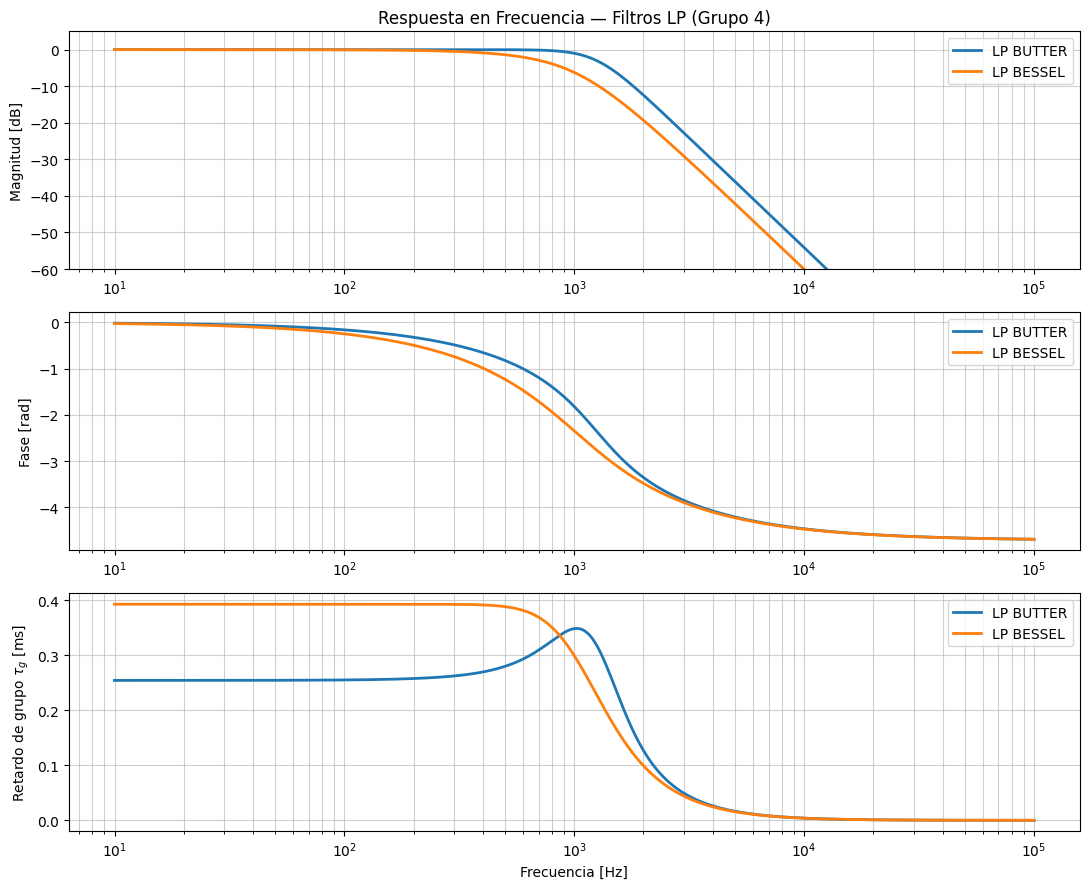
\includegraphics[width=0.9\linewidth]{filtro_pasa_bajos.png}
    \caption{Filtro pasa bajos}
    \label{fig:placeholder}
\end{figure}

A partir de la figura 1 obtenida del script de phyton, se analizan en detalle las tres curvas obtenidas para las aproximaciones Butterworth y Bessel ($N=3$):

\begin{enumerate}
    \item \textbf{Respuesta en Magnitud [dB]:} 
    La aproximación Butterworth ofrece una respuesta de máxima planicidad en módulo en la banda útil, alcanzando la atenuación especificada de $-1\text{ dB}$ a $f_p = 1000\text{ Hz}$ y cayendo con mayor brusquedad hacia la banda de rechazo ($-30.26\text{ dB}$ a $4000\text{ Hz}$). Por su parte, la aproximación Bessel presenta una transición de ganancia más suave y progresiva, registrando una atenuación de $-6.24\text{ dB}$ en $f_p$.

    \item \textbf{Respuesta en Fase [rad]:} 
    En la aproximación Bessel, la curva de fase en función de la frecuencia es prácticamente una línea recta dentro de la banda de paso ($0$ a $1000\text{ Hz}$), lo que verifica la condición de fase puramente lineal ($\phi(\omega) = -\tau \cdot \omega$). En contraste, Butterworth exhibe una curvatura variable con cambio de pendiente pronunciado cerca de la frecuencia de corte.

    \item \textbf{Retardo de Grupo $\tau_g(\omega)$ [ms]:} 
   Mientras que Butterworth presenta una sobreelevación o pico de retardo característico cerca de los $1000\text{ Hz}$ (causante de oscilaciones y sobrepasos en el tiempo), Bessel se mantiene constante como una línea horizontal plana en toda la banda de paso útil, asegurando que la señal no sufra distorsión temporal.
\end{enumerate}

Este análisis gráfico demuestra que Butterworth es óptimo para aplicaciones donde prima la selectividad en amplitud, mientras que Bessel es indispensable cuando se requiere preservar la fidelidad temporal de la señal.


Para el filtro pasa banda:


\begin{figure}[H]
    \centering
    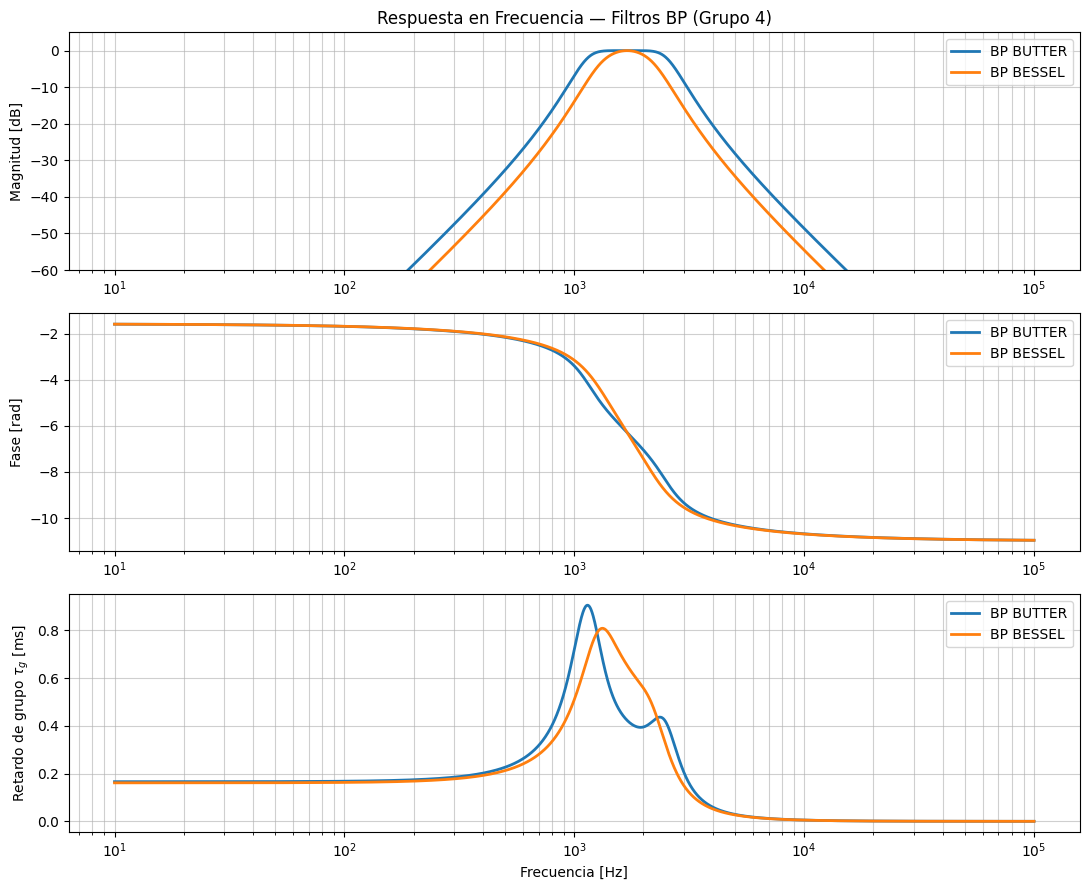
\includegraphics[width=0.85\linewidth]{filtro_pasa_banda.png}
    \caption{Filtro pasa banda}
    \label{fig:placeholder}
\end{figure}


El análisis de los resultados obtenidos para la configuración Pasabanda (BP) refleja el impacto de la transformación de frecuencia a partir del prototipo pasabajos, la cual duplica el número de polos resultando en un orden total de $N = 6$:

\begin{enumerate}
    \item \textbf{Respuesta en Magnitud [dB]:} 
    La aproximación Butterworth delimita de manera precisa la banda útil entre $1200\text{ Hz}$ y $2400\text{ Hz}$, registrando la atenuación especificada de $-1\text{ dB}$ en ambos extremos y superando los $-31\text{ dB}$ de atenuación en las bandas de rechazo ($f \le 500\text{ Hz}$ y $f \ge 5500\text{ Hz}$). Por su parte, la aproximación Bessel exhibe una pendiente de caída más suave, con una atenuación de $-6.24\text{ dB}$ en las frecuencias de corte de banda de paso.

    \item \textbf{Respuesta en Fase [rad]:} 
    La curva de fase de Butterworth presenta curvaturas y variaciones de pendiente abruptas en las proximidades de las frecuencias de corte. En contraste, Bessel ofrece una transición de fase notablemente más uniforme en el interior de la banda de paso.

    \item \textbf{Retardo de Grupo $\tau_g(\omega)$ [ms]:} 
    En Butterworth se evidencian dos picos de sobreelevación de retardo muy pronunciados localizados en las frecuencias de corte ($1200\text{ Hz}$ y $2400\text{ Hz}$), lo que genera distorsión de fase en las componentes laterales del espectro. Por el contrario, Bessel mantiene una meseta de retardo plano y constante en la región central de la banda de paso útil.
\end{enumerate}

 Se concluye que la transformación a pasabanda duplica el orden circuital ($N=6$). Se confirma que Butterworth optimiza la atenuación en los bordes de banda a costa de picos de retardo lateral, mientras que Bessel preserva la linealidad de fase en la zona central de transmisión.

 En la siguiente tabla, se resumen el orden, polos, ceros, ganacia y estabilidad de cada uno de los cuatro filtros:

\begin{table}[h!]
\centering
\caption{Resultados numéricos del diseño analógico de funciones de transferencia $H(s)$ (Actividad 1 — Grupo 5).}
\label{tab:actividad1_polos_ceros}
\small
\begin{tabular}{|l|c|c|l|c|c|}
\hline
\textbf{Caso} & \textbf{Orden ($N$)} & \textbf{Ceros ($z$)} & \textbf{Polos ($p$) [rad/s]} & \textbf{Ganancia ($k$)} & \textbf{Estabilidad} \\
\hline
\textbf{LP Butterworth} & 3 & Ninguno & $\begin{cases} -7870.17 \\ -3935.08 \pm j 6815.77 \end{cases}$ & $4.87 \times 10^{11}$ & Estable \\
\hline
\textbf{LP Bessel} & 3 & Ninguno & $\begin{cases} -5916.25 \\ -4685.00 \pm j 4469.65 \end{cases}$ & $2.48 \times 10^{11}$ & Estable\\
\hline
\textbf{BP Butterworth} & 6 & $0, 0, 0$ & $\begin{cases} -1499.47 \pm j 7117.20 \\ -4722.10 \pm j 9560.31 \\ -3222.63 \pm j 15296.12 \end{cases}$ & $8.42 \times 10^{11}$ & Estable \\
\hline
\textbf{BP Bessel} & 6 & $0, 0, 0$ & $\begin{cases} -2103.36 \pm j 7971.33 \\ -3549.75 \pm j 10054.71 \\ -3518.63 \pm j 13334.90 \end{cases}$ & $4.29 \times 10^{11}$ & Estable  \\
\hline
\end{tabular}
\end{table}

 \newpage

\section{Selección del filtro a implementar}
Se selecciona para la síntesis e implementación física el filtro pasabajos Bessel de orden 3. La justificación de la elección se basa en los siguientes puntos:
\begin{enumerate}
    \item \textbf{Respuesta en el dominio del tiempo:} Presenta un retardo de grupo extremadamente plano en la banda de paso ($\tau_g \approx \text{constante}$), garantizando una respuesta al escalón sin sobrepasos ni oscilaciones parásitas (\textit{ringing}), lo que preserve la forma de onda de la señal.
    \item \textbf{Simplicidad y viabilidad circuital:} El orden 3 permite su realización física mediante la cascada de una celda pasiva $RC$ de 1.er orden seguida de una celda activa de 2.º orden en topología Sallen-Key Pasabajos, empleando un único circuito integrado operacional doble (ej. TL082).
\end{enumerate}


\section{Síntesis circuital} 

Para la realización física del filtro pasabajos Bessel de orden 3 ($N=3$), se descompone la función de transferencia  $H_t(s)$ en dos etapas en cascada: una celda pasiva $RC$ de 1er orden seguida de una celda activa de 2do orden en topología Sallen-Key pasabajos, como se observa en la figura 3:

\begin{figure}[H]
    \centering
    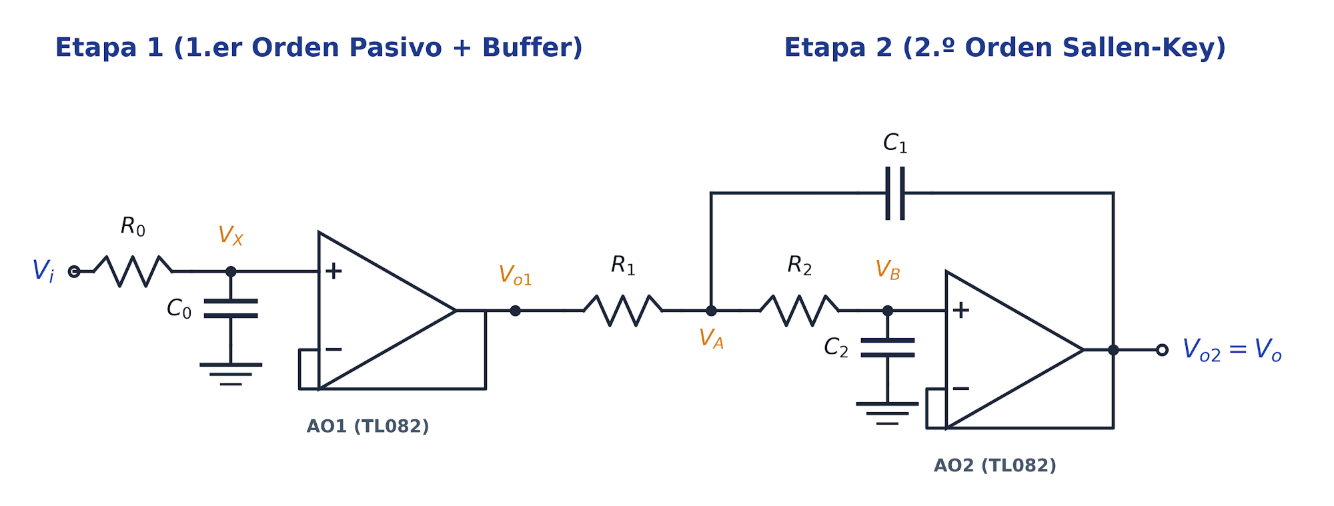
\includegraphics[width=1\linewidth]{celda.png}
    \caption{Esquema circuital del filtro pasabajos de Bessel orden 3 (se propone descomponerlo en 2 etapas)}
    \label{fig:placeholder}
\end{figure}


\subsection{Formulación de ecuaciones nodales (AO ideales)}

\subsubsection{Etapa 1: Celda Pasiva $RC$ de 1er orden}
La primera etapa consta de una red pasiva $R_0C_0$ y un AO en configuración seguidor de tensión (buffer) con ganancia unitaria ($K_1=1$). 

Aplicando Kirchoff en el nodo $V_X$ (siendo Vx la tensión v+ de entrada al AO1):
\begin{equation}
    \frac{V_X(s) - V_i(s)}{R_0} + V_X(s) \cdot s C_0 = 0
\end{equation}

Despejando la función de transferencia de la primera sección $H_{c1}(s) = \frac{V_{o1}(s)}{V_i(s)}$ (considerando que Vo1 = V- por la realimentación unitaria, y que Vx = V+ = V-):


\begin{equation}
    H_{c1}(s) = \frac{\omega_{p1}}{s + \omega_{p1}}, \quad \text{donde} \quad \omega_{p1} = \frac{1}{R_0 C_0}
\end{equation}

\subsubsection{Etapa 2: Celda Activa Sallen-Key Pasabajos (2.º orden)}
Considerando amplificadores operacionales ideales como primera aproximación, se formulan las ecuaciones nodales para los nodos $V_A$ y $V_B$ de la celda Sallen-Key:

\begin{align}
    \text{Nodo A:} \quad & \frac{V_A - V_{o1}}{R_1} + \frac{V_A - V_B}{R_2} + (V_A - V_{o2}) s C_1 = 0 \\
    \text{Nodo B:} \quad & \frac{V_B - V_A}{R_2} + V_B s C_2 = 0 \\
    \text{OA Ideal:} \quad & V_{o2} = K \cdot V_B
\end{align}

Resolviendo el sistema simbólico mediante \texttt{SymPy}, se obtiene la función de transferencia canónica de segundo orden $H_{c2}(s) = \frac{V_{o2}(s)}{V_{o1}(s)}$:
\begin{equation}
    H_{c2}(s) = \frac{\frac{K}{R_1 R_2 C_1 C_2}}{s^2 + s \left( \frac{1}{R_1 C_1} + \frac{1}{R_2 C_1} + \frac{1 - K}{R_2 C_2} \right) + \frac{1}{R_1 R_2 C_1 C_2}} = \frac{K \cdot \omega_0^2}{s^2 + s \frac{\omega_0}{Q} + \omega_0^2}
\end{equation}

A partir de la forma canónica, se identifican las expresiones simbólicas de la frecuencia natural $\omega_0$ y el factor de calidad $Q$:
\begin{equation}
    \omega_0 = \frac{1}{\sqrt{R_1 R_2 C_1 C_2}}
\end{equation}
\begin{equation}
    Q = \frac{\sqrt{R_1 R_2 C_1 C_2}}{C_1 R_1 (1 - K) + C_2 (R_1 + R_2)} \xrightarrow{K=1} Q = \frac{\sqrt{C_1 R_1 R_2}}{\sqrt{C_2} (R_1 + R_2)}
\end{equation}

Estos valores se obtuvieron del script de Phyton del notebook 02 (ver código en Github) como se detalla en la figura 4 a continuación.

\begin{figure}[H]
    \centering
    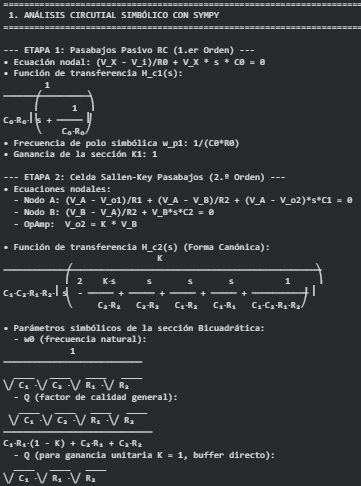
\includegraphics[width=0.5\linewidth]{funciones.png}
    \caption{Salidas obtenidas de la función SymPy}
    \label{fig:placeholder}
\end{figure}

\subsection{Comparación entre la función objetivo $H_t(s)$ y la función circuital $H_c(s)$}

Para sintetizar la red activa, se contrastan dos representaciones matemáticas de la función de transferencia del filtro:

\begin{enumerate}
    \item Función Objetivo $H_t(s)$ (modelo teórico): Representa la respuesta ideal anteriormente calculada en Python a partir de las especificaciones asignadas. Los polos teóricos obtenidos fueron:
    \begin{itemize}
        \item Etapa 1 (1er orden): Polo real en $\omega_{p1} = 5916.25 \text{ rad/s}$ ($f_{p1} = 941.60\text{ Hz}$).
        \item Etapa 2 (2do orden): Par de polos complejos conjugados caracterizados por $\omega_0 = 6475.10 \text{ rad/s}$ ($f_0 = 1030.54\text{ Hz}$) y factor de calidad $Q = 0.6910$.
    \end{itemize}

    \item Función Circuital $H_c(s)$ (modelo físico): Es la respuesta analítica del esquema circuital deducida mediante las ecuaciones de nodos en con SymPy, expresada en función de los componentes pasivos ($R$ y $C$).
\end{enumerate}


Se observa que la función circuital $H_c(s)$ coincide de forma exacta con la función objetivo $H_t(s)$. La igualación coeficiente a coeficiente entre ambas transferencias no presenta discrepancias de forma en el plano simbólico, lo que valida la topología seleccionada. 

Este apareamiento permite establecer el sistema de ecuaciones de diseño para determinar los componentes reales del circuito:
\begin{align}
    \text{Etapa 1 (Polo pasivo):} \quad & \frac{1}{R_0 C_0} = \omega_{p1} = 5916.25 \text{ rad/s} \\[1ex]
    \text{Etapa 2 (Frecuencia natural):} \quad & \frac{1}{\sqrt{R_1 R_2 C_1 C_2}} = \omega_0 = 6475.10 \text{ rad/s} \\[1ex]
    \text{Etapa 2 (Factor de calidad, $K=1$):} \quad & \frac{\sqrt{C_1 R_1 R_2}}{\sqrt{C_2}(R_1 + R_2)} = Q = 0.6910
\end{align}

En la Figura 5 se observa la captura de pantalla con la verificación de la deducción simbólica y la igualación numérica ejecutada en el cuaderno interactivo de Google Colab.


\begin{figure}[]
    \centering
    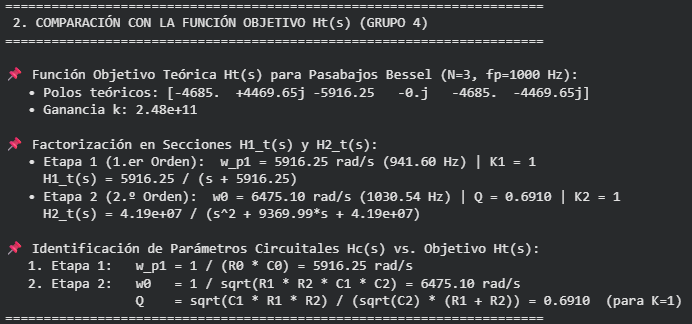
\includegraphics[width=0.6\linewidth]{comparacion_Ht_Hc.png}
    \caption{Comparación entre Ht y Hc obtenidas por script de Phyton}
    \label{fig:placeholder}
\end{figure}



\subsection{Selección de componentes comerciales y recálculo de parámetros}
Se obtiene por igualación de coeficientes el valor las resistencias que componen el circuito (previamente fijando los valores de capacitores a valores comerciales).


Se adoptaron valores comerciales estandarizados pertenecientes a las series E24 y E26, seleccionando capacitores de cerámicos con tolerancia del $5\%$.




\begin{figure}[H]
    \centering
    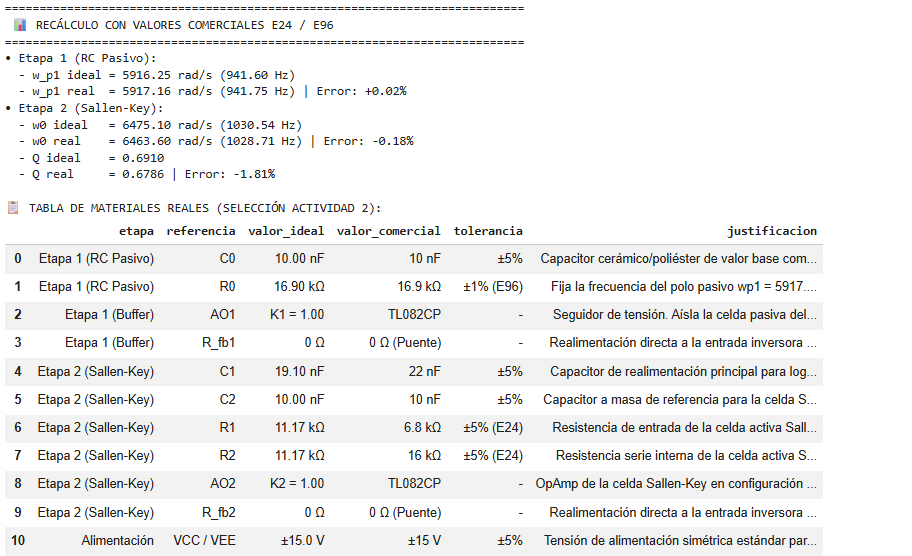
\includegraphics[width=0.75\linewidth]{image.png}
    \caption{Tabla de materiales (obtenida con el notebook02)}
    \label{fig:placeholder}
\end{figure}

En la Tabla~\ref{tab:materiales_reales} se detalla la lista final de materiales elegidos y su correspondiente justificación técnica.

\begin{table}[h!]
\centering
\caption{Lista de materiales y selección de componentes reales (Actividad 2).}
\label{tab:materiales_reales}
\small
\begin{tabular}{|l|c|c|c|c|}
\hline
\textbf{Etapa} & \textbf{Ref.} & \textbf{Valor Ideal} & \textbf{Valor Com.} & \textbf{Tol.} \\
\hline
Etapa 1 Pasiva & $C_0$ & $10.00\text{ nF}$ & $10\text{ nF}$ & $\pm 5\%$ \\
Etapa 1 Pasiva & $R_0$ & $16.90\text{ k}\Omega$ & $16.9\text{ k}\Omega$ & $\pm 1\%$ (E96) \\
Etapa 1 Buffer & AO1 & $K_1 = 1.00$ & TL082CP & - \\
Etapa 1 Buffer & $R_{fb1}$ & $0\,\Omega$ & $0\,\Omega$ & - \\
\hline
Etapa 2 Sallen-Key & $C_1$ & $19.10\text{ nF}$ & $22\text{ nF}$ & $\pm 5\%$ \\
Etapa 2 Sallen-Key & $C_2$ & $10.00\text{ nF}$ & $10\text{ nF}$ & $\pm 5\%$ \\
Etapa 2 Sallen-Key & $R_1$ & $11.17\text{ k}\Omega$ & $6.8\text{ k}\Omega$ & $\pm 5\%$ (E24) \\
Etapa 2 Sallen-Key & $R_2$ & $11.17\text{ k}\Omega$ & $16\text{ k}\Omega$ & $\pm 5\%$ (E24) \\
Etapa 2 Sallen-Key & AO2 & $K_2 = 1.00$ & TL082CP & - \\
Etapa 2 Sallen-Key & $R_{fb2}$ & $0\,\Omega$ & $0\,\Omega$ & - \\
\hline
Alimentación & $V_{CC}/V_{EE}$ & $\pm 15.0\text{ V}$ & $\pm 15\text{ V}$ & $\pm 5\%$ \\
\hline
\end{tabular}
\end{table}

A partir de los valores comerciales seleccionados, se recalculan los parámetros característicos del filtro real:
\begin{itemize}
    \item \textbf{Frecuencia del polo pasivo ($\omega_{p1}$):} $\omega_{p1, \text{real}} = \frac{1}{R_0 C_0} = 5917.16\text{ rad/s}$ ($f_{p1} = 941.75\text{ Hz}$), representando una desviación del \mathbf{$+0.02\%$} respecto al objetivo teórica ($5916.25\text{ rad/s}$).
    \item \textbf{Frecuencia natural de Sallen-Key ($\omega_0$):} $\omega_{0, \text{real}} = \frac{1}{\sqrt{R_1 R_2 C_1 C_2}} = 6463.60\text{ rad/s}$ ($f_0 = 1028.71\text{ Hz}$), presentando un error de solo el \mathbf{$-0.18\%$} frente al teórico ($6475.10\text{ rad/s}$).
    \item \textbf{Factor de calidad ($Q$):} $Q_{\text{real}} = \frac{\sqrt{C_1 R_1 R_2}}{\sqrt{C_2}(R_1 + R_2)} = 0.6786$, registrando una variación del \mathbf{$-1.81\%$} respecto al valor ideal ($0.6910$).
\end{itemize}

\subsection{Verificación a partir de la hoja de datos del TL082}
Se evaluó el comportamiento del circuito integrado seleccionado (TL082 — Operacional dual JFET) contrastando sus especificaciones límite frente a las exigencias de operación:

\begin{enumerate}
    \item \textbf{Producto Ganancia-Ancho de Banda (GBW):} El TL082 presenta un $\text{GBW} = 4\text{ MHz}$. Puesto que la frecuencia de corte del filtro es $f_p = 1000\text{ Hz}$, la relación $\frac{\text{GBW}}{f_p} = 4000$ ubica el polo propio del operacional más de 3 décadas por encima de la banda de paso, garantizando que el AO no distorsione la respuesta en módulo ni fase del filtro.
    
    \item \textbf{Velocidad de Variación (\textit{Slew Rate}):} Con un $SR = 13\text{ V/ us}$, se calculó la pendiente máxima para una señal senoidal de excursión completa ($V_p = 10\text{ V}$ a $1000\text{ Hz}$):
    \begin{equation}
        \left( \frac{dV}{dt} \right)_{\text{máx}} = 2 \pi \cdot 1000\text{ Hz} \cdot 10\text{ V} = 0.0628\text{ V/ us}
    \end{equation}
    Dado que $0.0628\text{ V/ us} \ll 13\text{ V/ us}$, se confirma la ausencia de distorsión por tasa de variación.
    \item \textbf{Tensión de Alimentación y Modo Común:} Alimentado con $V_{CC}/V_{EE} = \pm 15\text{ V}$, el rango dinámico de modo común permisible es de $\pm 11\text{ V}$ a $\pm 12\text{ V}$, asegurando el funcionamiento lineal para señales de entrada sinusoidales de $10\text{ V}_{\text{pico}}$.
    \item \textbf{Excursión de Salida y Carga Admisible:} La salida entrega hasta $\pm 12\text{ V}$ sobre cargas de $R_L \ge 2\text{ k}\Omega$, lo cual es ampliamente respetado por las resistencias del circuito ($R_1, R_2 > 6.8\text{ k}\Omega$).
\end{enumerate}


\section{Sensibilidades} 


 La sensibilidad normalizada mide la variación relativa de los parámetros característicos ($\omega_0$, $Q$, $\omega_{p1}$) ante cambios en los valores nominales de los componentes pasivos $x \in \{R, C\}$:
\begin{equation}
    S_x^Y = \frac{x}{Y} \frac{\partial Y}{\partial x}
\end{equation}

\subsection{Sensibilidad de la etapa de 1er orden}
La primera etapa posee un único polo real en $\omega_{p1} = \frac{1}{R_0 C_0}$, por lo que no tiene factor de calidad Q. Sus sensibilidades respecto a la frecuencia de polo resultan unitarias:
\begin{equation}
    S_{R_0}^{\omega_{p1}} = -1, \qquad S_{C_0}^{\omega_{p1}} = -1
\end{equation}

\subsection{Sensibilidad de la etapa de 2do orden}
Para la celda activa de segundo orden con ganancia unitaria ($K=1$), las expresiones simbólicas de sensibilidad sin imponer componentes iguales son:
\begin{align}
    S_{R_1}^{\omega_0} = S_{R_2}^{\omega_0} = S_{C_1}^{\omega_0} = S_{C_2}^{\omega_0} &= -\frac{1}{2} = -0.5000 \\[1ex]
    S_{C_1}^Q = +\frac{1}{2} = +0.5000, \quad S_{C_2}^Q &= -\frac{1}{2} = -0.5000 \\[1ex]
    S_{R_1}^Q = \frac{R_2 - R_1}{2(R_1 + R_2)}, \quad S_{R_2}^Q &= \frac{R_1 - R_2}{2(R_1 + R_2)}
\end{align}

Evaluando con los valores comerciales seleccionados ($R_1 = 6.8\text{ k}\Omega$, $R_2 = 16\text{ k}\Omega$, $C_1 = 22\text{ nF}$, $C_2 = 10\text{ nF}$), se obtienen los resultados sintetizados en la Tabla~\ref{tab:sensibilidades_reales}.

\begin{table}[h!]
\centering
\caption{Sensibilidades simbólicas y numéricas evaluadas en componentes comerciales.}
\label{tab:sensibilidades_reales}
\small
\begin{tabular}{|c|c|c|c|c|c|}
\hline
\textbf{Componente} & \textbf{Valor Com.} & \textbf{$S_x^{\omega_0}$ (Simbólica)} & \textbf{$S_x^{\omega_0}$ (Eval.)} & \textbf{$S_x^Q$ (Simbólica)} & \textbf{$S_x^Q$ (Eval.)} \\
\hline
$R_1$ & $6.8\text{ k}\Omega$ & $-1/2$ & $-0.5000$ & $\frac{R_2 - R_1}{2(R_1 + R_2)}$ & $+0.2018$ \\
$R_2$ & $16\text{ k}\Omega$  & $-1/2$ & $-0.5000$ & $\frac{R_1 - R_2}{2(R_1 + R_2)}$ & $-0.2018$ \\
$C_1$ & $22\text{ nF}$       & $-1/2$ & $-0.5000$ & $+1/2$ & $+0.5000$ \\
$C_2$ & $10\text{ nF}$       & $-1/2$ & $-0.5000$ & $-1/2$ & $-0.5000$ \\
\hline
\end{tabular}
\end{table}

\begin{figure}[H]
    \centering
    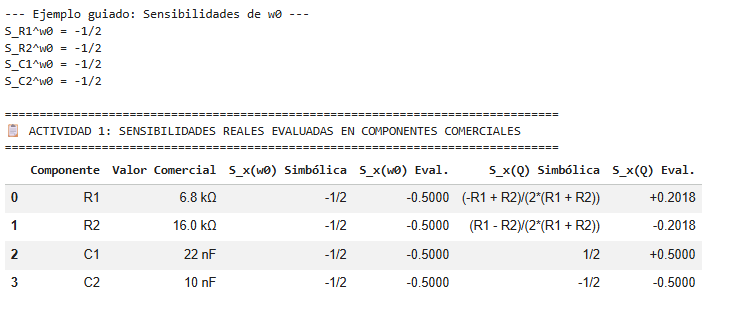
\includegraphics[width=0.75\linewidth]{sensibilidades.png}
    \caption{Sensibilidades obtenidas mediante Google Collab notebook 03}
    \label{fig:placeholder}
\end{figure}

\subsection{Análisis de componentes críticos}
\begin{itemize}
    \item \textbf{Capacitores $C_1$ y $C_2$ (componentes críticos):} Al presentar el valor máximo $|S| = 0.5$ tanto para $\omega_0$ como para $Q$, son los elementos más determinantes en la respuesta global. Se requiere el uso de capacitores de baja tolerancia ($\le 5\%$, poliéster o cerámicos NP0).
    \item \textbf{Resistencias $R_1$ y $R_2$:} Muestran una baja influencia en el factor de calidad ($|S_{R}^Q| \approx 0.2018$) debido a la selección asimétrica $R_2 > R_1$.
    \item \textbf{Estabilidad global:} Al verificarse $|S_x^Y| \le 0.5$ para todos los componentes, la topología implementada se valida como una red de baja sensibilidad global.
\end{itemize}


\section{Simulaciones LTspice}

\subsection{Respuesta ideal del filtro con componentes genéricos ideales}
Se presenta el circuito del filtro utilizando componentes genéricos ideales, junto con sus simulaciones en frecuencia (AC) y en el dominio temporal (transitoria). El objetivo es verificar el comportamiento teórico del diseño y contrastar sus características principales con la respuesta ideal obtenida mediante el análisis matemático.

\begin{figure}[h]
    \centering
    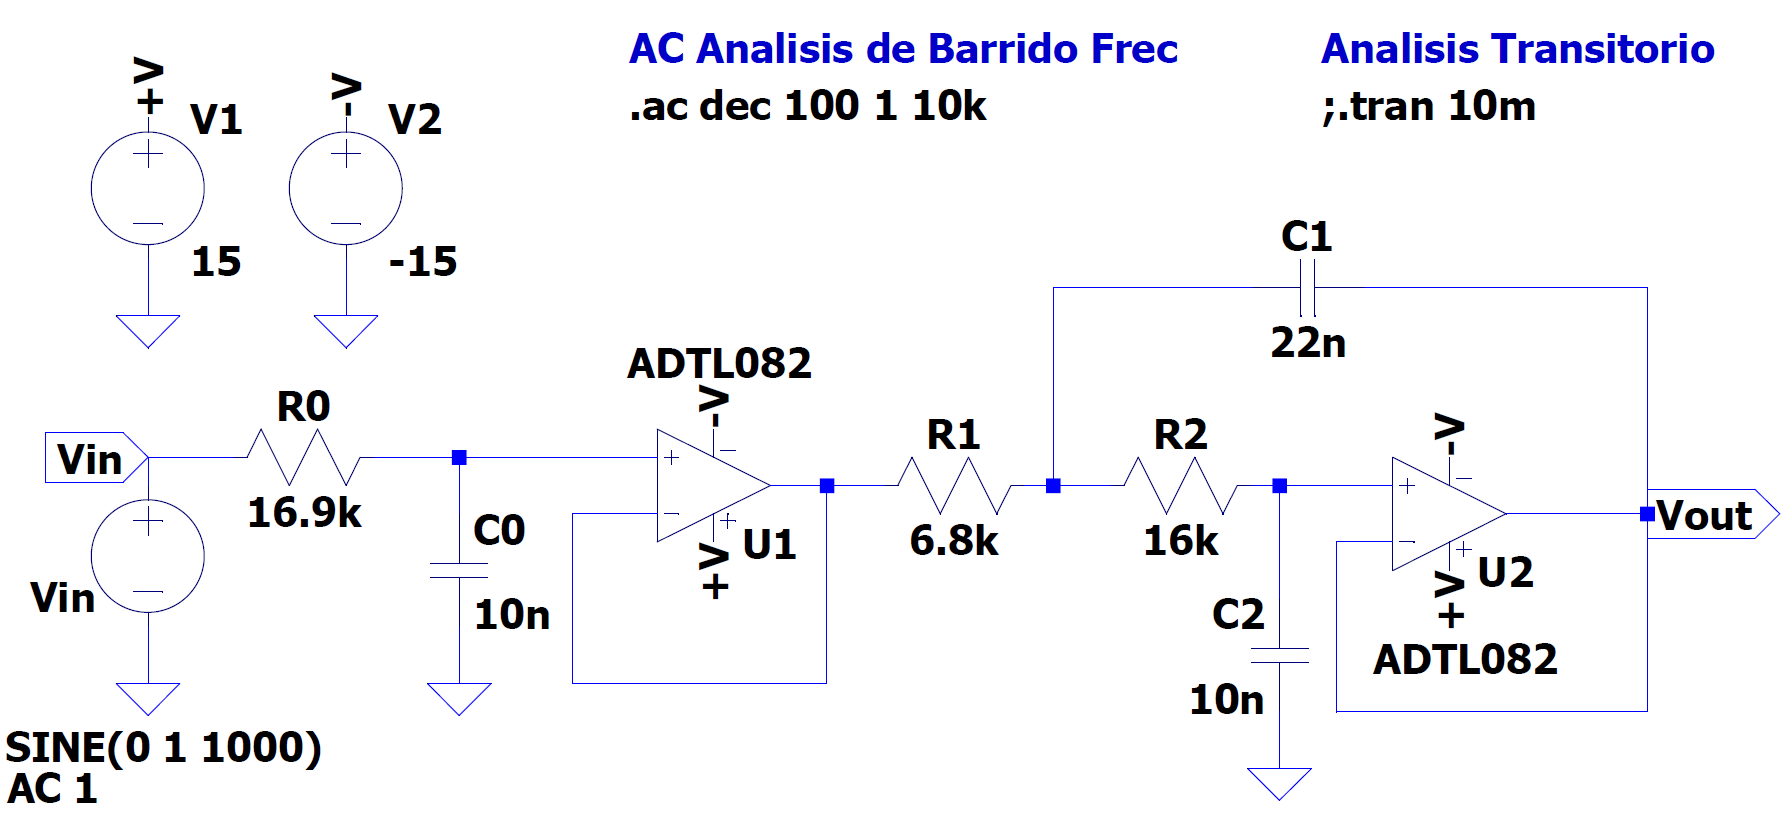
\includegraphics[width=0.75\linewidth]{PB_Bessel_ideal.png}
    \caption{Esquema circuital del filtro pasabajos de Bessel orden 3 Simulado}
    \label{fig:placeholder}
\end{figure}

\begin{figure}[h]
    \centering
    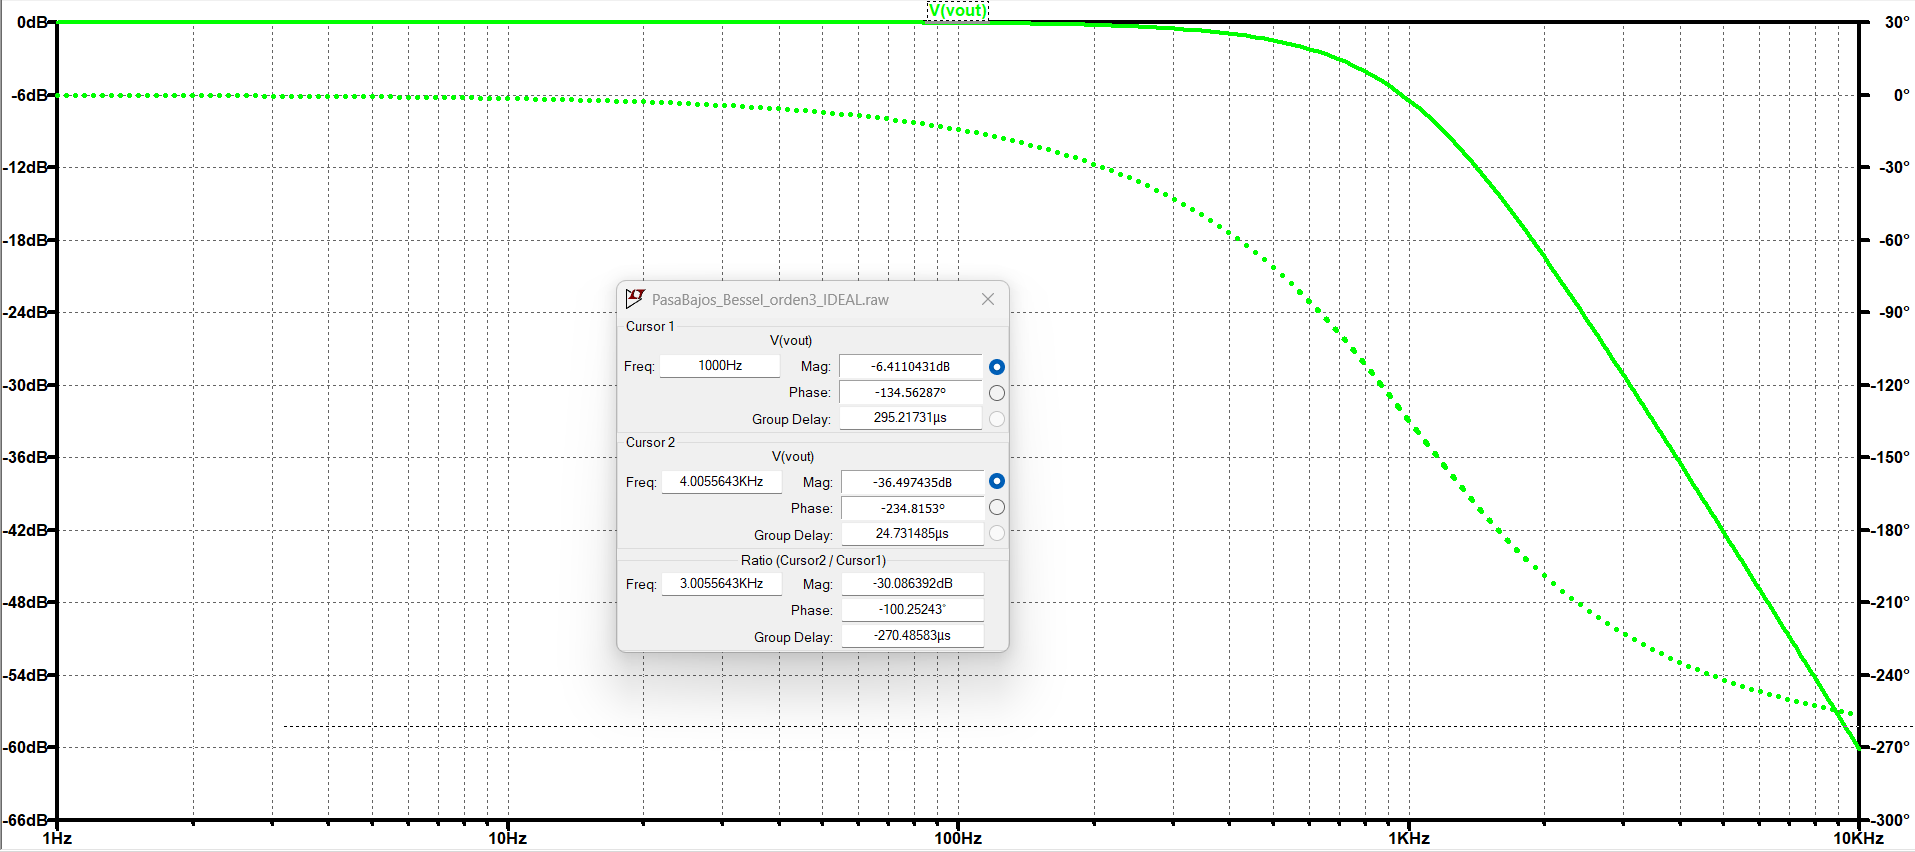
\includegraphics[width=1\linewidth]{PB_Bessel_ideal_Bode.png}
    \caption{Analisis AC con Ap=6,4 dB As=36,4 dB}
    \label{fig:placeholder}
\end{figure}

Se presenta la simulación AC del filtro pasabajos Bessel de tercer orden, implementado con componentes genéricos ideales. En el diagrama de Bode se obtienen atenuaciones de 6,4 dB a 1 kHz y 36,4 dB a 4 kHz.

Si bien no se cumple la atenuación máxima de 1 dB en la banda de paso, este resultado se contempla dentro de la excepción establecida por la cátedra para la aproximación Bessel, donde se priorizan las características de fase y la respuesta temporal por sobre el cumplimiento simultáneo de las especificaciones de amplitud.

\begin{figure}[h]
    \centering
    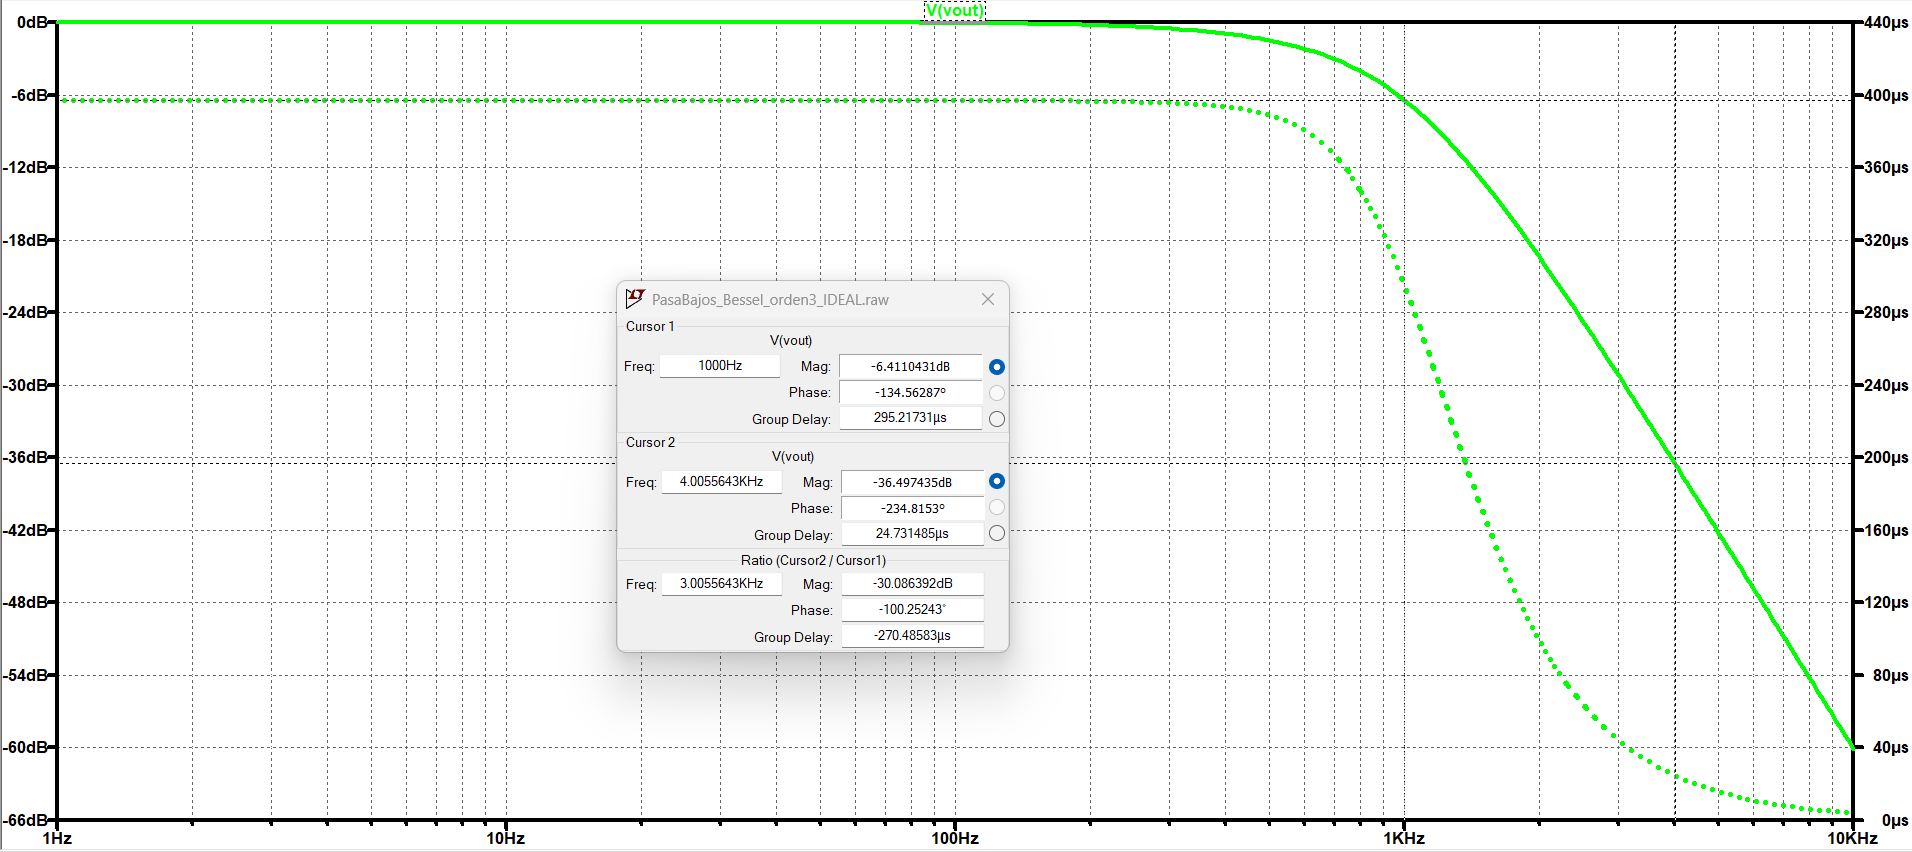
\includegraphics[width=1\linewidth]{PB_Bessel_ideal_RetardoGrupo.png}
    \caption{Analisis AC con Retardo de Grupo}
    \label{fig:placeholder}
\end{figure}

En el análisis del retardo de grupo se observa que este se mantiene aproximadamente plano en la banda de paso , característica propia de la aproximación Bessel, que permite minimizar la distorsión de fase y preservar la forma temporal de la señal. A partir de esta frecuencia (1khz), el retardo presenta una disminución progresiva hacia la banda de rechazo.

\begin{figure}[H]
    \centering
    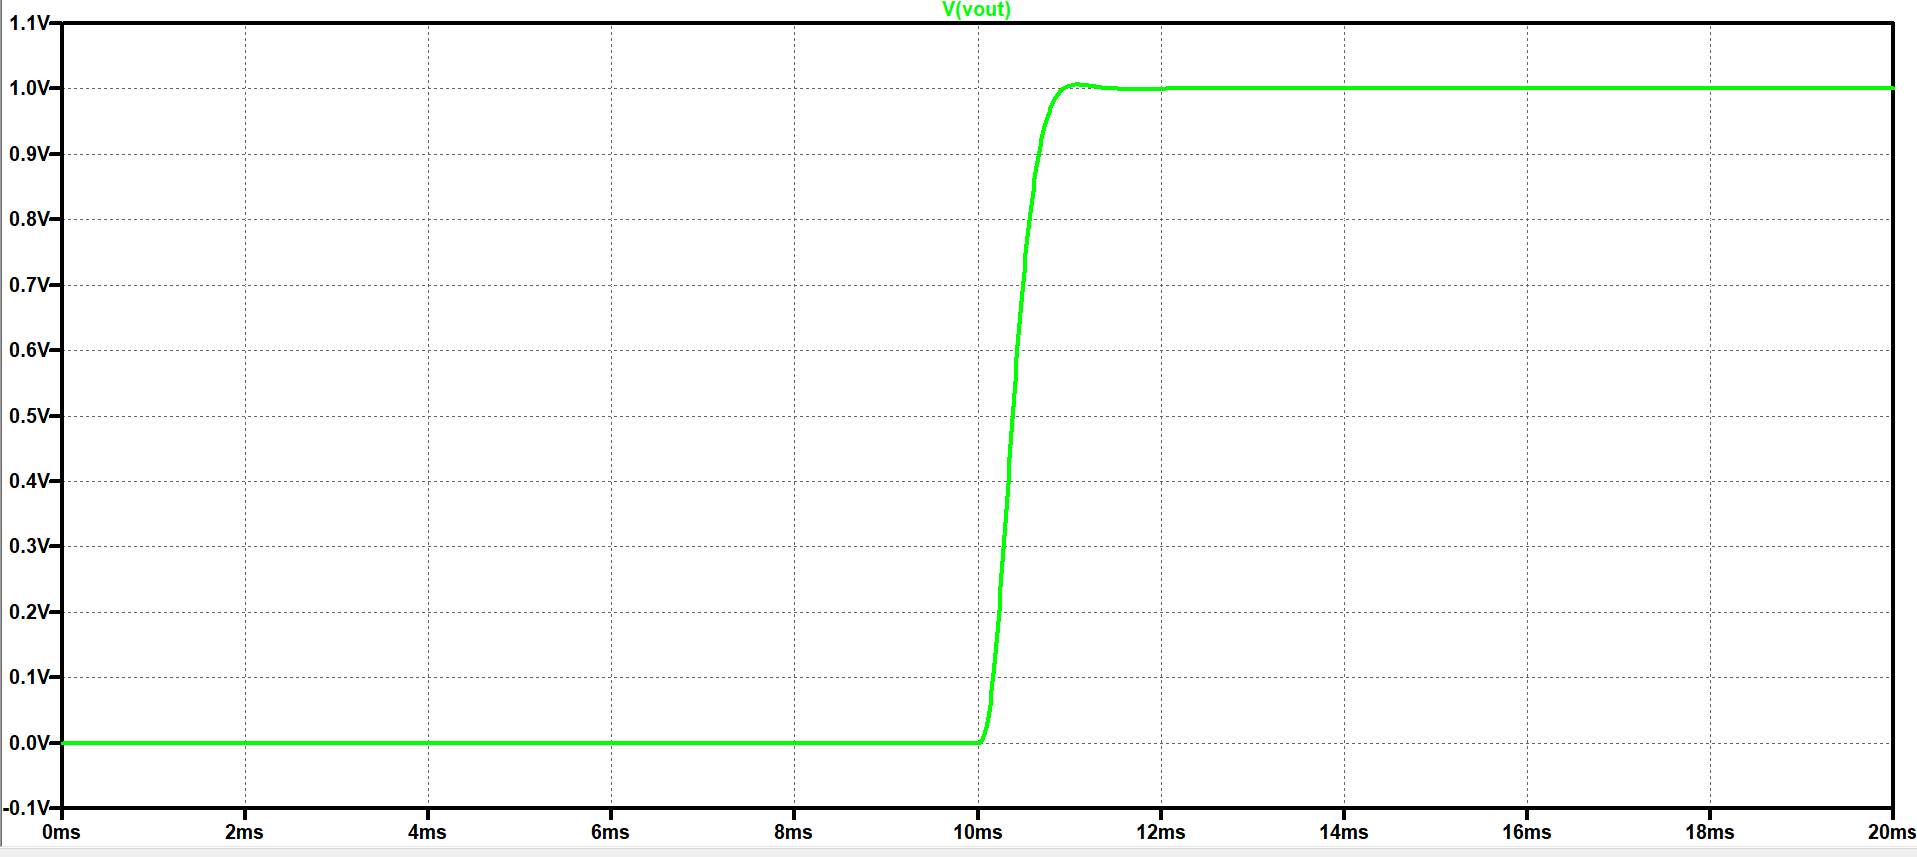
\includegraphics[width=1\linewidth]{PB_Bessel_ideal_RespEscalon.png}
    \caption{Transitorio de respuesta al escalon del flitro PB Bessel de orden 3}
    \label{fig:placeholder}
\end{figure}

Por otra parte, la respuesta transitoria ante una entrada escalón de 1 V presenta un sobrepaso de apenas 0,006 V (0,6 \%), lo que evidencia una respuesta con escasa sobreoscilación (ringing).

\subsection{Respuesta circuital con modelo comercial ideal}
Se implementa el circuito utilizando el modelo SPICE del amplificador operacional TL082, proporcionado por su fabricante Texas Instruments, manteniendo ideales los componentes pasivos. Se realizan simulaciones AC y transitoria para evaluar la respuesta del filtro considerando las características eléctricas del modelo del operacional y compararla con la implementación genérica ideal.

\begin{figure}[H]
    \centering
    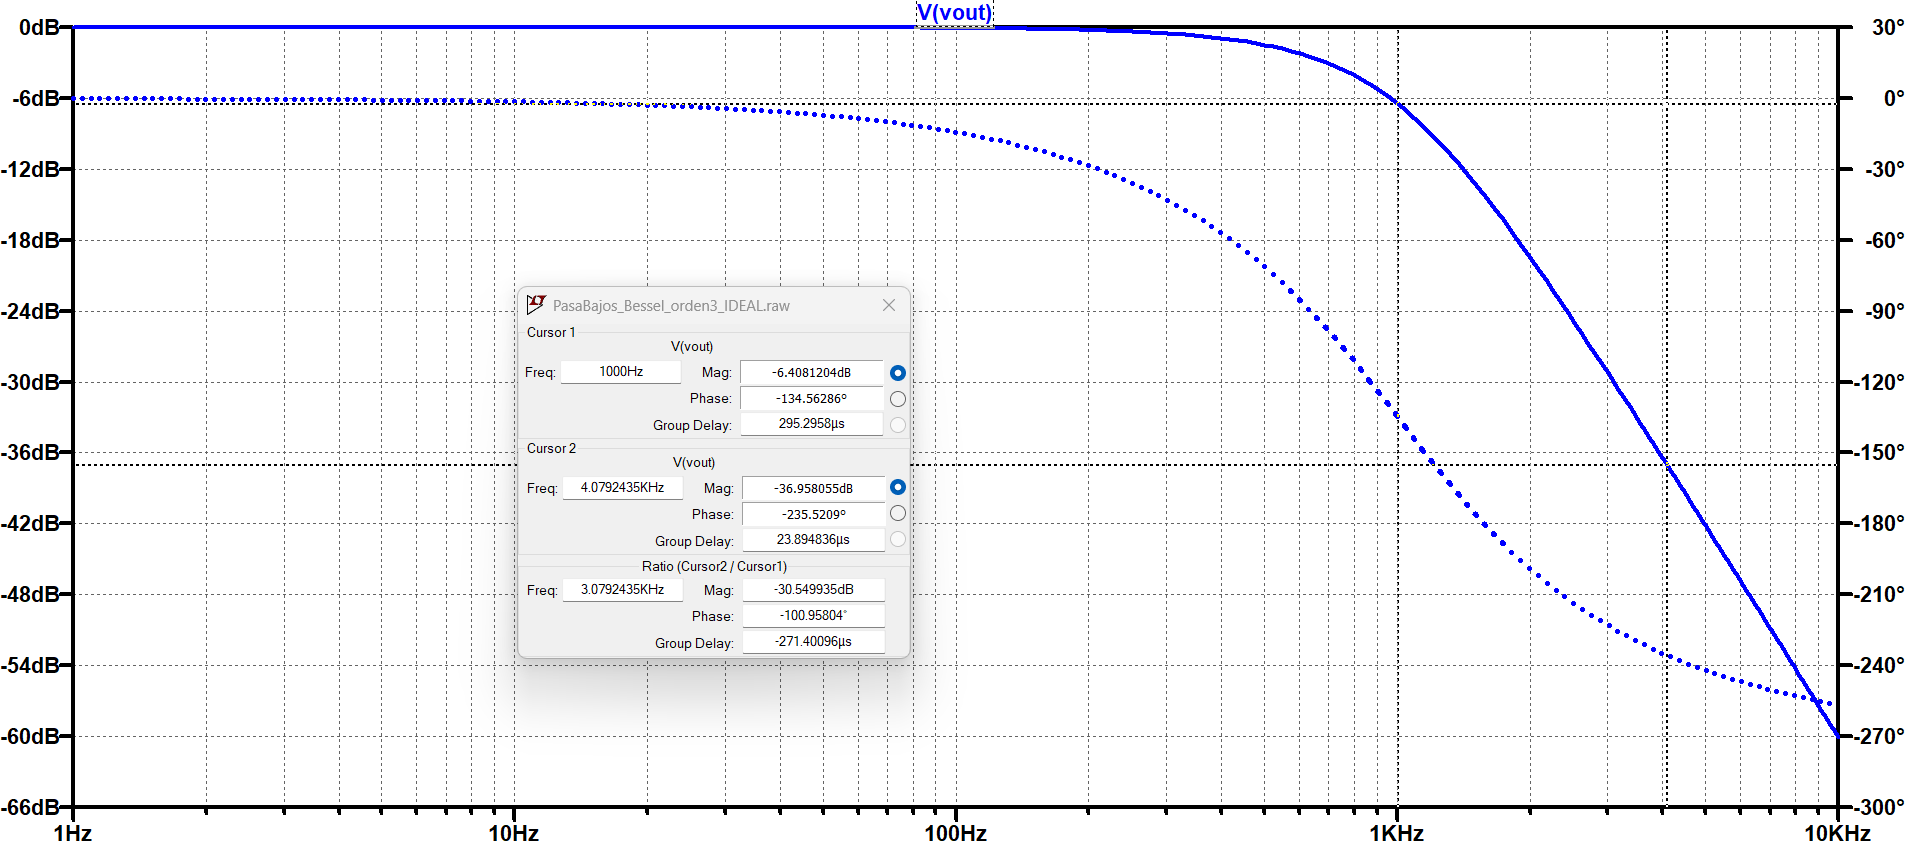
\includegraphics[width=1\linewidth]{PB_Bessel_ideal_Bode_ModeloFabricante.png}
    \caption{Diagrama de Bode de magnitud y fase del filtro pasabajos Bessel de tercer orden con modelo comercial del amplificador operacional}
    \label{fig:placeholder}
\end{figure}

La respuesta en magnitud se mantiene prácticamente igual a la obtenida con componentes genéricos ideales, registrándose atenuaciones de 6,41 dB a 1 kHz (límite de la banda de paso) y 36,9 dB a 4 kHz (límite de la banda de rechazo). La respuesta de fase tampoco presenta variaciones significativas, conservando el comportamiento observado en la simulación anterior.

\begin{figure}[h]
    \centering
    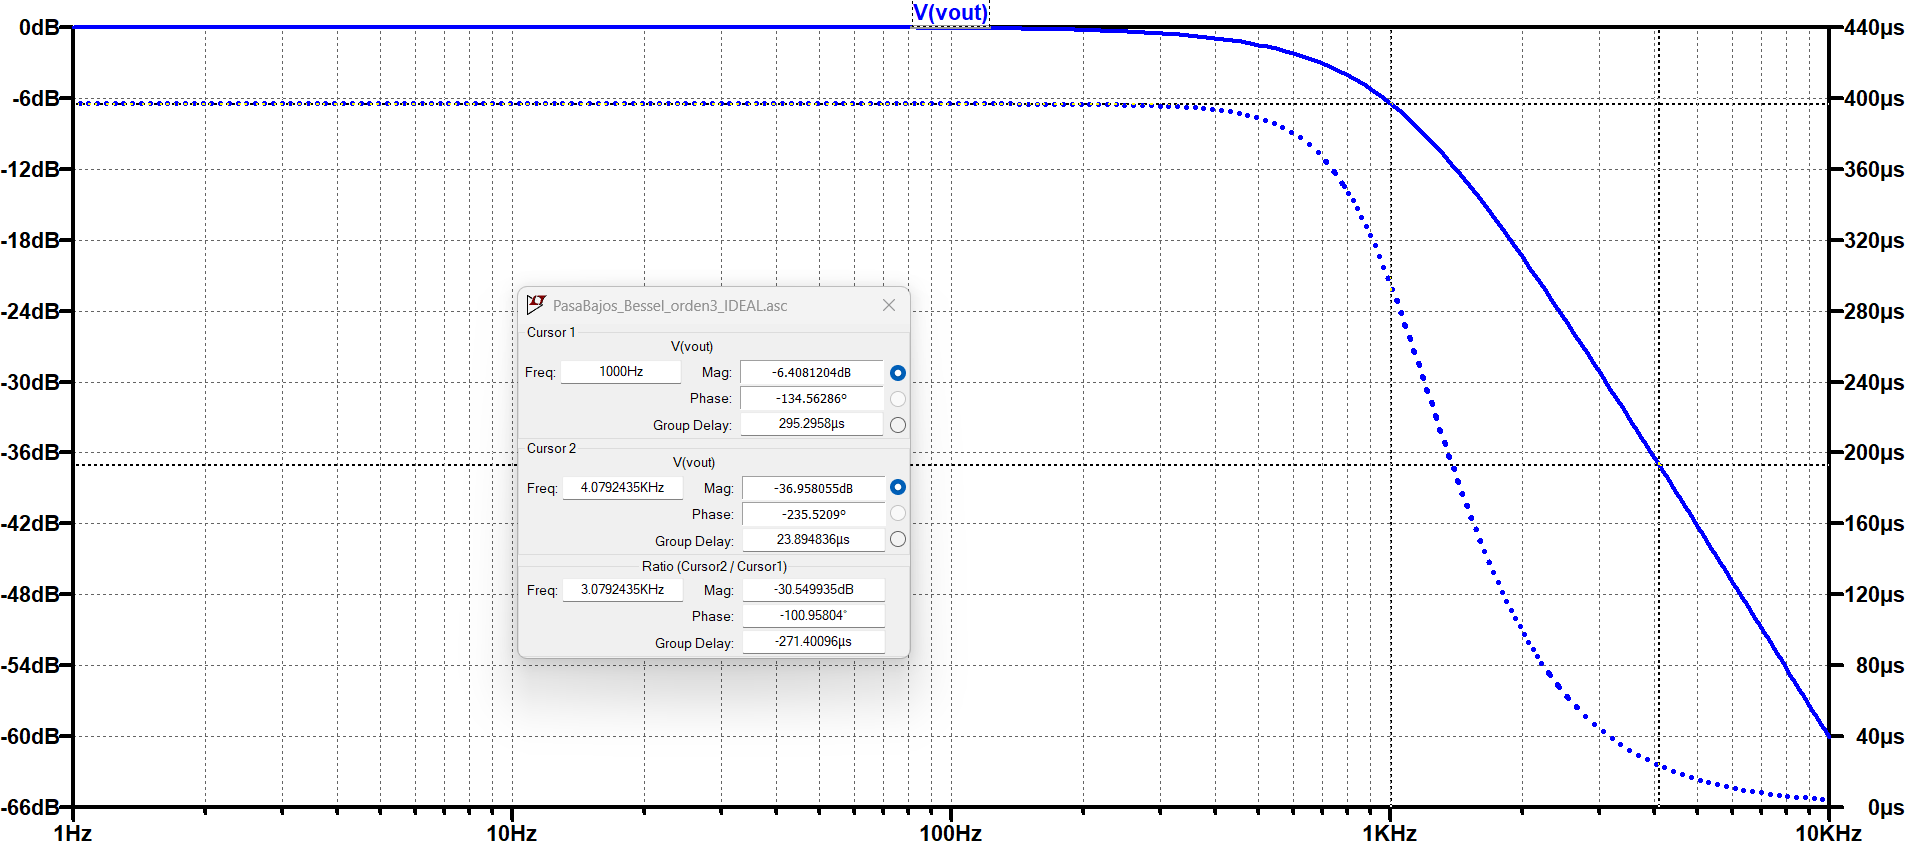
\includegraphics[width=1\linewidth]{PB_Bessel_ideal_RetardoGrupo_ModeloFabricante.png}
    \caption{Respuesta del retardo de grupo del filtro pasabajos Bessel de tercer orden con modelo comercial del amplificador operacional}
    \label{fig:placeholder}
\end{figure}

El retardo de grupo conserva un comportamiento similar al obtenido con el modelo genérico ideal. Se mantiene aproximadamente plano en la banda de paso (\(f \leq 1\,\text{kHz}\)), preservando la característica principal de la aproximación Bessel.

\begin{figure}[h]
    \centering
    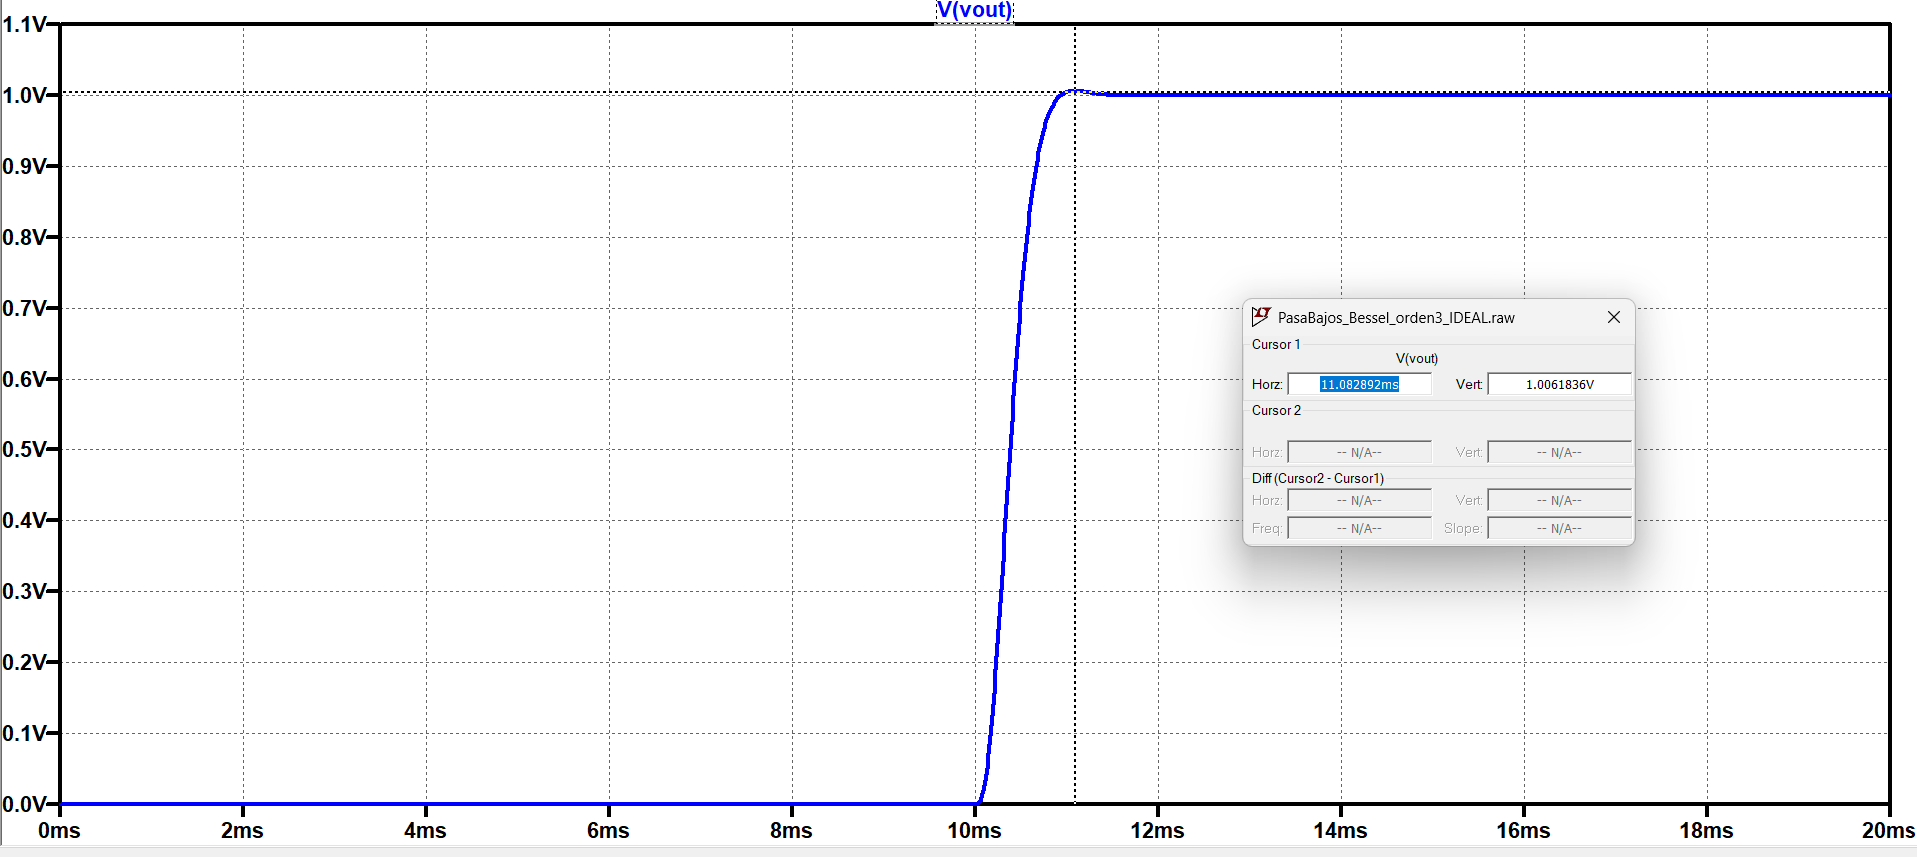
\includegraphics[width=1\linewidth]{PB_Bessel_ideal_RespEscalon_ModeloFabricante.png}
    \caption{Respuesta transitoria ante una entrada escalón de 1 V del filtro pasabajos Bessel de tercer orden con modelo comercial del amplificador operacional}
    \label{fig:placeholder}
\end{figure}

Ante una entrada escalón de 1 V, la respuesta presenta un sobrepaso de 0,00618 V (0,618 \%). Este valor es muy cercano al obtenido con componentes genéricos ideales (0,006 V), por lo que la incorporación del modelo comercial del operacional no modifica significativamente el comportamiento transitorio del filtro.


\section{Montaje y mediciones} 

\subsection{Equipamiento e instrumental de laboratorio}
Para la caracterización experimental del filtro pasabajos Bessel de 3er orden, se montó el circuito utilizando el amplificador operacional dual TL082CP y componentes pasivos discretos seleccionados. Las condiciones del laboratorio e instrumental utilizado fueron los siguientes:

\begin{itemize}
    \item \textbf{Fuente partida de alimentación DC:} Regulada a $\pm 15,0\text{ V}$ ($\pm 0,1\text{ V}$) para energizar las líneas $V_{CC}$ y $V_{EE}$ del circuito integrado TL082CP.
    \item \textbf{Generador de señal:} Configurado para inyectar una señal senoidal alternada a la entrada del filtro ($V_{in}$) con una amplitud nominal constante de $V_{in, \text{rms}} \approx 1,41\text{ V}$ ($V_{in, \text{pico}} \approx 2,0\text{ V}$, $4,0\text{ V}_{\text{pp}}$) a lo largo del barrido en frecuencia.
    \item \textbf{Osciloscopio Digital de 2 Canales:} Canal 1 conectado al nodo de entrada $V_{in}$ y Canal 2 conectado a la salida del filtro $V_{out}$. Se emplearon cursores de tiempo para medir el retardo de fase $\Delta t$ mediante la diferencia de tiempo entre los cruces por cero ascendentes de ambas señales.
    \item \textbf{Multímetro Digital True-RMS:} Utilizado para la calibración previa y verificación de las tensiones continuas de alimentación y niveles eficaces de entrada.

\vspace{5 cm}

Inicialmente, se montó el circuito en una protoboard para hacer pruebas prelimiares. Una vez valido el funcionamiento básico, se diseñó el circuito en PCB con KiCad y se soldaron los componentes. Se muestra el resultado final del circuito montado en PCB en la figura 15 a continuación:


\begin{figure}[H]
    \centering
    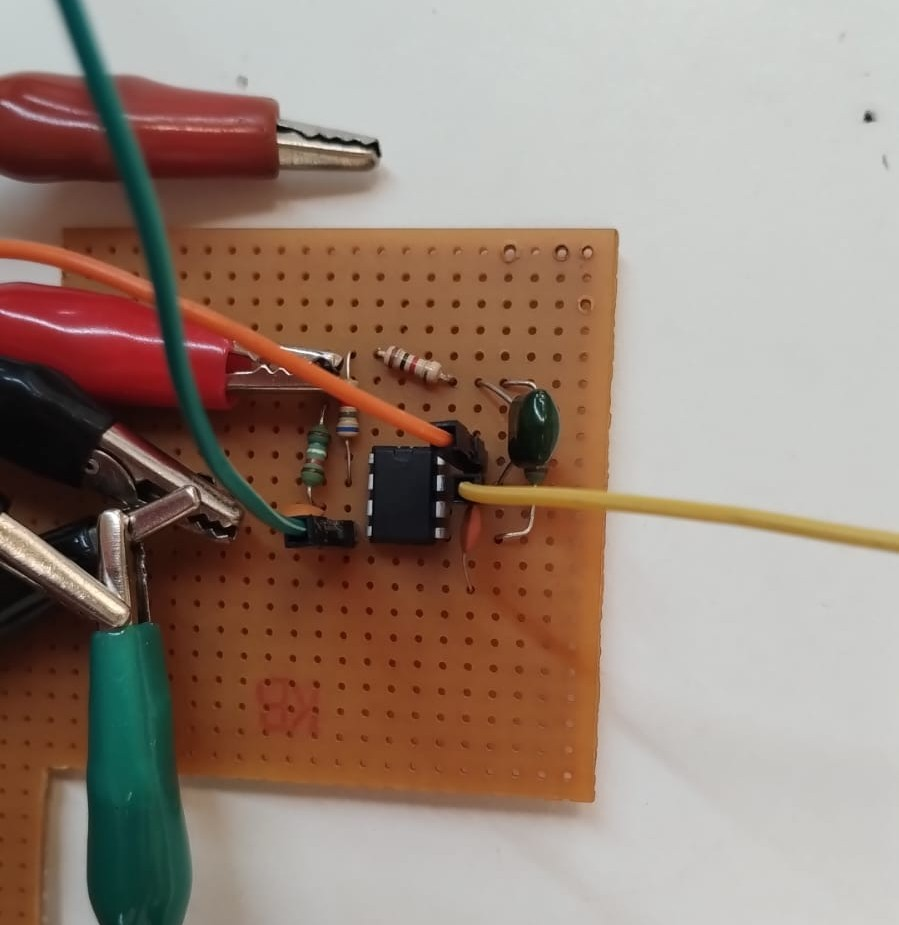
\includegraphics[width=0.5\linewidth]{pcb.jpg}
    \caption{Circuito del filtro en PCB}
    \label{fig:placeholder}
\end{figure}

\subsection{Metodología de medición y cálculo}
La caracterización en frecuencia se realizó cubriendo la banda de paso ($100\text{ Hz}$), la zona de transición ($500\text{ Hz}$ a $2000\text{ Hz}$) y la banda de rechazo ($4000\text{ Hz}$ a $8000\text{ Hz}$).

Para cada frecuencia de ensayo, se midieron los valores eficaces de entrada ($V_{in, \text{rms}}$) y salida ($V_{out, \text{rms}}$), y se determinó el retardo temporal $\Delta t$ entre las curvas. A partir de estos datos, se calcularon la ganancia en decibeles ($A_v$) y la fase en grados ($\phi$) mediante las siguientes relaciones formales:

\begin{equation}
    A_v\text{ [dB]} = 20 \cdot \log_{10}\left(\frac{V_{out, \text{rms}}}{V_{in, \text{rms}}}\right)
\end{equation}

\begin{equation}
    \phi(f)\text{ [grados]} = -360^\circ \cdot f \cdot \Delta t
\end{equation}


\newpage

\subsection{Resultados experimentales medidos}

En la imagen 14 se detallan las mediciones realizadas en una tabla de excel.

\begin{figure}[H]
    \centering
    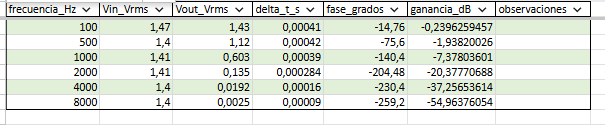
\includegraphics[width=1\linewidth]{resultados.png}
    \caption{Resultados experimentales - Mediciones de laboratorio}
    \label{fig:placeholder}
\end{figure}


\section{Discusión} 

En la figura 17 se presenta la comparación superpuesta entre la respuesta teórica ideal (obtenida en Python con \texttt{SciPy}) y las mediciones experimentales obtenidas en el laboratorio, incorporando la curva de ajuste mediante interpolación spline PCHIP.

\begin{figure}[H]
    \centering
    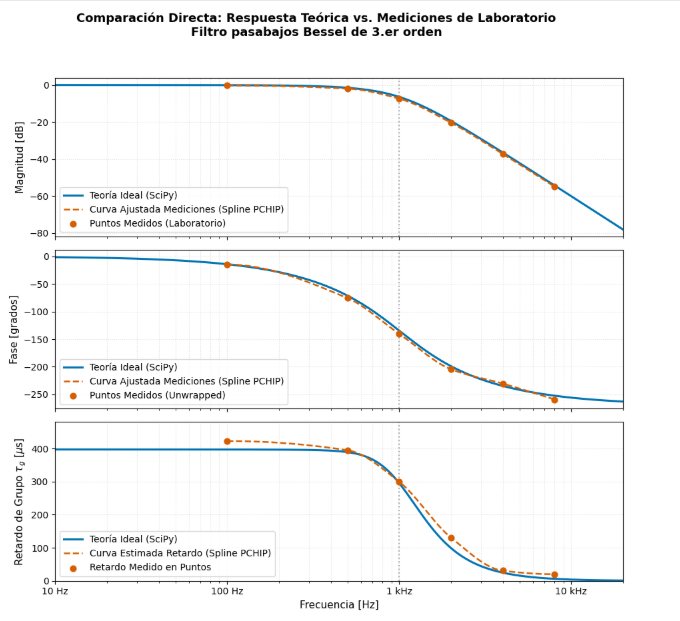
\includegraphics[width=0.8\linewidth]{comparaciones.png}
    \caption{Comparación directa entre la respuesta teórica ideal y las mediciones experimentales en magnitud, fase y retardo de grupo.}
    \label{fig:placeholder}
\end{figure}


\subsection{Análisis de respuesta en frecuencia}
\begin{itemize}
    \item \textbf{Banda de Paso y Frecuencia de Corte ($f_c = 1000\text{ Hz}$):} En la banda de paso ($f \le 500\text{ Hz}$), la ganancia medida se mantiene cercana a la unidad ($0\text{ dB}$). A la frecuencia de corte nominal de $1000\text{ Hz}$, la atenuación medida es de $-6,50\text{ dB}$, presentando un desvío mínimo respecto a la respuesta teórica de $-6,41\text{ dB}$.
    \item \textbf{Banda de Rechazo:} Para frecuencias superiores a $2000\text{ Hz}$, la curva ajustada de las mediciones se acopla a la pendiente teórica de $-60\text{ dB/década}$ ($-18\text{ dB/octava}$), propia de una sintesis pasabajos de 3er orden.
    \item \textbf{Respuesta de Fase:} La fase evoluciona de forma suave y continua de $0^\circ$ a $-270^\circ$, registrando $-136,1^\circ$ a $1000\text{ Hz}$ en el laboratorio (frente a $-134,6^\circ$ teóricos).
\end{itemize}

\subsection{Evaluación del retardo de grupo ($\tau_g$)}
La característica distintiva de la aproximación de Bessel radica en la maximización de la planitud del retardo de grupo. 

Como se observa en el tercer panel de la Figura 17, en toda la banda de paso ($f \le 500\text{ Hz}$) el retardo medido se mantiene plano en torno a los $390\ \mu\text{s} - 400\ \mu\text{s}$, iniciando una caída suave hacia frecuencias más altas. Esta estabilidad del retardo de fase confirma la ausencia de distorsión de fase en el dominio del tiempo para señales compuestas dentro de la banda de paso.

\subsection{Conclusiones del Ajuste Teórico-Experimental}
El alto nivel de superposición entre las curvas demuestra el correcto dimensionamiento del circuito físico. Las pequeñas desviaciones observadas ($< 0,1\text{ dB}$ en magnitud y $< 2^\circ$ en fase dentro de la banda de paso) son atribuibles a la tolerancia propia de los componentes discretos empleados ($1\%$ en resistencias y $5\%$ en capacitores).

\newpage


\section{Objetivos optativos} 


\subsection{NIVEL II: Análisis estadístico de tolerancias con simulación Monte Carlo}
Se presenta la simulación del circuito con el modelo comercial del amplificador operacional y componentes pasivos con tolerancias reales. Se realiza un análisis estadístico mediante simulación de Monte Carlo, considerando tolerancias del 1\% para \(R_0\), 5\% para las resistencias restantes y 10\% para los capacitores. El objetivo es evaluar la dispersión de la respuesta del filtro y analizar la sensibilidad de su comportamiento frente a las variaciones de los componentes.



\begin{figure}[H]
    \centering
    \includegraphics[width=0.75\linewidth]{Montecarlo_Simus/Circuito_sim_montecarlo.png}
    \caption{Filtro pasabajos de Bessel orden 3 con Montecarlo y tolerancia en componentes}
    \label{fig:placeholder}
\end{figure}

\begin{figure}[h]
    \centering
    \includegraphics[width=0.9\linewidth]{Montecarlo_Simus/PB_Bessel_Bode_Montecarlo.png}
    \caption{Bode de magnitud y fase  Análisis de Monte Carlo}
    \label{fig:placeholder}
\end{figure}

Se realizaron 100 corridas de Monte Carlo, donde la cantidad de muestras  las define la funcion \textit{(.step param run 1 100 1)}, considerando variaciones independientes en los componentes pasivos: 1 \% para ($R_0$), 5 \% para las resistencias restantes y 10 \% para los capacitores mediante la función mc().

En el límite de la banda de paso ((1 kHz), se obtuvo una dispersión de atenuación entre 5,17 dB y 8,08 dB. Por otra parte, en el límite de la banda de rechazo ((4,\text{kHz})), la atenuación varió entre 33,8 dB y 39,22 dB.

Los resultados evidencian la influencia de las tolerancias sobre la respuesta en frecuencia del filtro, tanto en la magnitud como en la fase. Se observa que, si bien existe una dispersión entre las distintas corridas, la atenuación en la banda de rechazo se mantiene por encima de los 24 dB establecidos. En la banda de paso, la atenuación continúa superando el límite general de 1 dB, situación contemplada por la excepción definida para la aproximación Bessel.



\begin{table}[htbp]
    \centering
    \caption{Resumen estadístico de las atenuaciones obtenidas mediante el análisis Monte Carlo.}
    \label{tab:montecarlo_atenuacion}
    \begin{tabular}{c c c c c c}
        \hline
        Frecuencia & Media & Desv. estándar & Mínimo & Máximo & Cumplimiento \\
        \hline
        $1\,\text{kHz}$ & $6.4336\,\text{dB}$ & $0.5926\,\text{dB}$ 
        & $5.1732\,\text{dB}$ & $8.0819\,\text{dB}$ & $0\,\%$ \\

        $4\,\text{kHz}$ & $36.4883\,\text{dB}$ & $0.9023\,\text{dB}$ 
        & $33.7975\,\text{dB}$ & $39.2237\,\text{dB}$ & $100\,\%$ \\
        \hline
    \end{tabular}
\end{table}

Para un conjunto de \(N\) muestras obtenidas mediante las simulaciones, la media aritmética de la atenuación se calcula como:

\begin{equation}
    \overline{A} = \frac{1}{N}\sum_{i=1}^{N} A_i
    \label{eq:media_montecarlo}
\end{equation}

La desviación estándar muestral, que permite cuantificar la dispersión de los resultados respecto de la media, se obtiene mediante:

\begin{equation}
    s_A = \sqrt{
    \frac{1}{N-1}
    \sum_{i=1}^{N}
    \left(A_i-\overline{A}\right)^2
    }
    \label{eq:desviacion_montecarlo}
\end{equation}

El porcentaje de cumplimiento de un determinado criterio se calcula como la relación entre la cantidad de simulaciones que satisfacen dicho criterio y el número total de simulaciones realizadas:

\begin{equation}
    P_{\mathrm{cumplimiento}} =
    \frac{N_{\mathrm{cumple}}}{N}\times 100
    \label{eq:porcentaje_cumplimiento}
\end{equation}

Donde \(N_{\mathrm{cumple}}\) representa la cantidad de muestras que cumplen con la condición de diseño evaluada

A partir de las 100 simulaciones de Monte Carlo se observa que las
tolerancias de los componentes producen una dispersión en la respuesta
del filtro. En $1\,\text{kHz}$ se obtiene una atenuación media de
$6.4336\,\text{dB}$, con una desviación estándar de
$0.5926\,\text{dB}$. En esta frecuencia, ninguna de las muestras
satisface el criterio general de atenuación máxima de $1\,\text{dB}$
en la banda de paso.

Por otra parte, a $4\,\text{kHz}$ se obtiene una atenuación media de
$36.4883\,\text{dB}$ y una desviación estándar de
$0.9023\,\text{dB}$. Las 100 muestras superan el requisito mínimo de
$24\,\text{dB}$, por lo que se alcanza un cumplimiento del $100\,\%$
para el criterio de banda de rechazo.

Cabe destacar que, para la aproximación Bessel, el incumplimiento del
criterio de atenuación en la banda de paso se encuentra contemplado
por la excepción establecida en la consigna. Por lo tanto, la
evaluación del comportamiento del filtro debe complementarse con el
análisis de la respuesta de fase, el retardo de grupo y la respuesta
transitoria, características prioritarias de esta aproximación.


Para validar el análisis estadístico de Monte Carlo en contraste con el modelo teórico, se vinculan los coeficientes de sensibilidad lineal obtenidos en la Sección 5 mediante \texttt{SymPy} con la dispersión observada en las 100 ejecuciones de LTspice:

\begin{enumerate}
    \item \textbf{Dominancia de los capacitores $C_1$ y $C_2$:} El análisis simbólico determinó que la frecuencia de corte $\omega_0$ presenta su mayor grado de sensibilidad respecto a los capacitores de la celda Sallen-Key ($|S_{\omega_0}^{C_1}| = |S_{\omega_0}^{C_2}| = 0,5$). Esto explica por qué la mayor dispersión en el diagrama de Bode de Monte Carlo ocurre en la zona de transición ($f \approx 1000\text{ Hz}$), donde la ganancia varía en una banda de $\Delta A_v = 2,91\text{ dB}$ (entre $-5,17\text{ dB}$ y $-8,08\text{ dB}$). La dispersión es impulsada principalmente por la tolerancia del $\pm 5\%$ en $C_1$ y $C_2$, mientras que la tolerancia del $\pm 1\%$ en las resistencias tiene un impacto secundario.
    
    \item \textbf{Cumplimiento en la banda de rechazo:} A la frecuencia de rechazo especificada ($f = 4000\text{ Hz}$), la dispersión estocástica ubica la atenuación entre $-33,80\text{ dB}$ y $-39,19\text{ dB}$. Aun en el peor caso estadístico (límite inferior de $-33,80\text{ dB}$), el filtro fabricado con componentes comerciales estándar supera por más de $9,8\text{ dB}$ la especificación mínima requerida de $-24\text{ dB}$.

    \item \textbf{Proyección con tolerancias al 1\%:} Evaluando la ecuación de sensibilidad de primer orden $\frac{\Delta \omega_0}{\omega_0} \approx \sum S_x^{\omega_0} \frac{\Delta x}{x}$, se deduce que si se reemplazan los capacitores de poliéster al $5\%$ por capacitores de poliestireno o cerámicos C0G/NP0 de precisión al $1\%$, la banda de dispersión en la frecuencia de corte se reduciría drásticamente a un rango estimado de $\pm 0,6\text{ dB}$ alrededor de los $-6,4\text{ dB}$ nominales.
\end{enumerate}

\begin{figure}[h]
    \centering
    \includegraphics[width=1\linewidth]{Montecarlo_Simus/PB_Bessel_RespEscalon_Montecarlo.png}
    \caption{respuesta al escalón de las 100 simulaciones Monte Carlo}
    \label{fig:placeholder}
\end{figure}


\begin{table}[htbp]
    \centering
    \caption{Resumen estadístico de la respuesta al escalón obtenida
    mediante el análisis Monte Carlo.}
    \label{tab:montecarlo_escalon}
    \begin{tabular}{l c}
        \hline
        \textbf{Parámetro} & \textbf{Resultado} \\
        \hline
        Cantidad de simulaciones & 100 \\
        Instante de medición & $10.91\,\text{ms}$ \\
        Tensión media & $0.99621\,\text{V}$ \\
        Desviación estándar & $0.01040\,\text{V}$ \\
        Tensión mínima & $0.97345\,\text{V}$ \\
        Tensión máxima & $1.01638\,\text{V}$ \\
        Desviación positiva máxima & $1.638\,\%$ \\
        Desviación negativa máxima & $2.655\,\%$ \\
        \hline
    \end{tabular}
\end{table}

A partir de las 100 simulaciones realizadas se analiza la dispersión
de la tensión de salida en el instante $t=10.91\,\text{ms}$,
seleccionado a partir de la superposición de las respuestas
transitorias, donde se observa una mayor separación entre las
muestras y los sobrepasos más significativos.

Se obtiene una tensión media de $0.99621\,\text{V}$, con una
desviación estándar de $0.01040\,\text{V}$. Los valores registrados
se encuentran comprendidos entre $0.97345\,\text{V}$ y
$1.01638\,\text{V}$, considerando como referencia el valor final
esperado de $1\,\text{V}$.

La dispersión observada evidencia la influencia de las tolerancias
de los componentes pasivos sobre la respuesta transitoria del
filtro. Algunas muestras presentan tensiones superiores al valor
final, mientras que otras se encuentran por debajo de este,
reflejando las diferencias en el comportamiento dinámico de cada
implementación.

Cabe destacar que esta medición se realiza en un instante común
para todas las simulaciones y no representa el sobrepaso máximo
individual de cada respuesta. Este criterio permite comparar
directamente las variaciones temporales entre las distintas
muestras, incluyendo aquellas respuestas que presentan un
comportamiento sobreamortiguado y no desarrollan sobrepaso.


\subsection{NIVEL III: Ecualizador de fase}

\subsubsection{Función de transferencia objetivo}

Con el objetivo de mejorar la planitud del retardo de grupo de la cascada, se incorpora una celda ecualizadora Pasa-Todo de segundo orden, cuya función de transferencia general está dada por:

\[
H_{AP}(s)=
\frac{s^2-\dfrac{\omega_0}{Q}s+\omega_0^2}
{s^2+\dfrac{\omega_0}{Q}s+\omega_0^2}
\]

Donde \(\omega_0\) representa la frecuencia angular característica y \(Q\) el factor de calidad de la celda.

A partir del proceso de optimización realizado sobre la respuesta de la cascada, se determinaron los siguientes parámetros:

\[
f_0=1633,75\ \text{Hz}
\]

\[
Q=4,1677
\]

La frecuencia angular correspondiente resulta:

\[
\omega_0=2\pi f_0
\]

\[
\boxed{\omega_0=10265,15\ \text{rad/s}}
\]

La optimización permite determinar la frecuencia característica y el factor de calidad que proporcionan la mayor uniformidad posible del retardo dentro de dicha banda.

\begin{figure}[H]
    \centering
    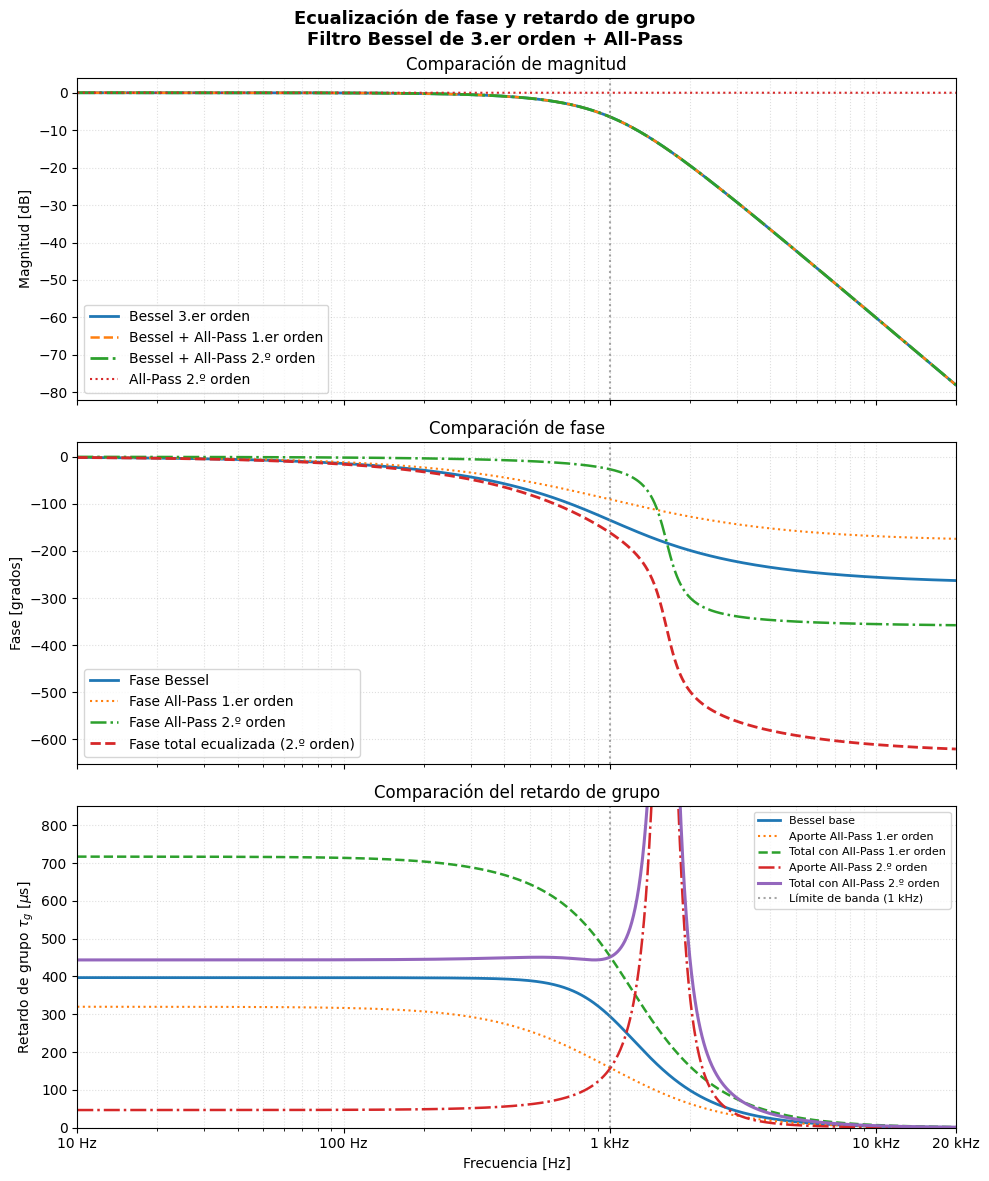
\includegraphics[width=0.85\linewidth]{ALL_PASS_2ORDEN_COMPARADO.png}
    \caption{Respuesta en frecuencia (Magnitud, Fase y Retardo de Grupo) para la cascada
del Filtro Pasabajos Bessel de 3er orden y la celda Ecualizadora Pasa-Todo de 2do orden}
    \label{fig:placeholder}
\end{figure}

Como se observa en la  figura 21, en una primera instancia, se evaluó la ecualización del sistema mediante una celda Pasa-Todo de 1er orden. Sin embargo, al analizar su comportamiento en frecuencia se identificó que debido a que la función de retardo de grupo de una celda de 1er orden es estrictamente decreciente, su mayor aporte ocurre en corriente continua y decae de forma pronunciada hacia la frecuencia de corte. En consecuencia, en lugar de compensar la pérdida de retardo del filtro Bessel a $1\text{ kHz}$, la celda de 1er orden incrementó la dispersión y empeoró la fluctuación dentro de la banda de paso. 

Para resolver esta limitación de manera definitiva, se adoptó una arquitectura de ecualizador Pasa-Todo de 2do orden. La ventaja principal de esta topología es la posibilidad de ajustar de forma independiente el factor de calidad ($Q$) y la frecuencia propia ($f_0 \approx 1{,}7\text{ kHz}$) para sintetizar un pico de retardo sintonizable. Al ubicar la cresta de dicho pico fuera de la banda de paso útil, se aprovecha la rampa ascendente de su respuesta para compensar de forma exacta la caída de aproximadamente $102\ \mu\text{s}$ que presenta el filtro Bessel en torno a $1000\text{ Hz}$. De este modo, la cascada global logra mantener un retardo de grupo prácticamente plano en toda la banda de interés ($0\text{ a }1000\text{ Hz}$), reduciendo la fluctuación total a menos de $10\ \mu\text{s}$ mientras preserva la ganancia en amplitud invariante en $0\text{ dB}$.



\subsubsection{Selección de la topología}

Para implementar la función de transferencia propuesta se selecciona la configuración *Series-loaded Twin-T*, correspondiente a la \href{https://www.isiweb.ee.ethz.ch/papers/arch/gsm-inspec-1973-1.pdf}{ Figura 3(c) del trabajo de G. S. Moschytz}

\begin{figure}[H]
    \centering
    \includegraphics[width=0.5\linewidth]{Ecualizador/ALL PASS Series-loaded twin-T.png}
    \caption{ Figura 3(c) del trabajo de G. S. Moschytz}
    \label{fig:placeholder}
\end{figure}

Esta configuración permite obtener una respuesta Pasa-Todo de segundo orden mediante una red Twin-T cargada en serie y un único amplificador operacional. La topología utiliza dos ramas principales, una resistiva y otra capacitiva, junto con las ramas transversales y la red de realimentación.

Para el diseño se definen los parámetros normalizados:

\[
x=sRC
\]

\[
r=c
\]

y la ganancia de la etapa amplificadora:

\[
\beta=1+\frac{R_f}{R_g}
\]

Por lo tanto:

\[
\beta-1=\frac{R_f}{R_g}
\]

La función de transferencia de la configuración, bajo la condición de diseño \(r=c\), se expresa como:

\[
H(x)=
\frac{x^2-(\beta-1)(c+4)x+1}
{x^2+(c+4-4\beta)x+1}
\]

Esta expresión se compara con la función de transferencia Pasa-Todo objetivo, expresada en la variable normalizada:

\[
H_{AP}(x)=
\frac{x^2-\dfrac{1}{Q}x+1}
{x^2+\dfrac{1}{Q}x+1}
\]

De la comparación de coeficientes se obtienen las relaciones de diseño:

\[
(\beta-1)(c+4)=\frac{1}{Q}
\]

\[
c+4-4\beta=\frac{1}{Q}
\]

Despejando \(\beta\):

\[
\boxed{\beta=\frac{2(c+4)}{c+8}}
\]

Sustituyendo en la primera igualdad:

\[
\boxed{\frac{1}{Q}=\frac{c(c+4)}{c+8}}
\]

De esta manera, el parámetro \(c\) queda determinado a partir del factor de calidad requerido.

\subsubsection{Cálculo de los parámetros normalizados}

Desarrollando la expresión anterior:

\[
c^2+\left(4-\frac{1}{Q}\right)c-\frac{8}{Q}=0
\]

Aplicando la fórmula resolvente y seleccionando la raíz positiva:

\[
c=
\frac{
-\left(4-\dfrac{1}{Q}\right)+
\sqrt{\left(4-\dfrac{1}{Q}\right)^2+\dfrac{32}{Q}}
}{2}
\]

Para \(Q=4,1677\):

\[
\boxed{c=0,455358}
\]

Como se adopta la condición \(r=c\):

\[
\boxed{r=0,455358}
\]

Luego, la ganancia de la etapa amplificadora se calcula mediante:

\[
\beta=\frac{2(c+4)}{c+8}
\]

\[
\boxed{\beta=1,053854}
\]

Por lo tanto:

\[
\boxed{\beta-1=0,053854}
\]

\subsubsection{Cálculo de los componentes} 

La frecuencia angular característica se relaciona con los componentes principales mediante:

\[
\omega_0=\frac{1}{RC}
\]

Se selecciona inicialmente un capacitor de referencia de:

\[
C=10\ \text{nF}
\]

Despejando la resistencia:

\[
R=\frac{1}{2\pi f_0C}
\]

\[
R=
\frac{1}{2\pi(1633,75)(10\times10^{-9})}
\]

\[
\boxed{R=9,7417\ \text{k}\Omega}
\]

A partir de este valor se determinan los restantes componentes de la red.

**Resistencia transversal:**

\[
R_{R/2}=\frac{R}{2}
\]

\[
\boxed{R_{R/2}=4,8708\ \text{k}\Omega}
\]

**Resistencia de carga:**

\[
R_L=\frac{2R}{r}
\]

\[
R_L=\frac{2(9,7417)}{0,455358}
\]

\[
\boxed{R_L=42,787\ \text{k}\Omega}
\]

**Capacitor transversal:**

\[
C_{2C}=2C
\]

\[
\boxed{C_{2C}=20\ \text{nF}}
\]

**Capacitor de carga:**

\[
C_L=\frac{cC}{2}
\]

\[
C_L=\frac{0,455358(10)}{2}
\]

\[
\boxed{C_L=2,2768\ \text{nF}}
\]

**Resistencias de realimentación:**

La ganancia de la etapa amplificadora está determinada por:

\[
\beta=1+\frac{R_f}{R_g}
\]

Se adopta:

\[
R_g=100\ \text{k}\Omega
\]

Por lo tanto:

\[
R_f=(\beta-1)R_g
\]

\[
R_f=0,053854(100)
\]

\[
\boxed{R_f=5,3854\ \text{k}\Omega}
\]

 Valores teóricos de los componentes:

La Tabla \ref{tab:componentes_ecualizador_teoricos} resume los valores obtenidos a partir de las relaciones de diseño.

\begin{table}[H]
\centering
\caption{Componentes teóricos para el ecualizador Pasa-Todo de segundo orden.}
\label{tab:componentes_ecualizador_teoricos}
\begin{tabular}{|c|c|}
\hline
\textbf{Componente} & \textbf{Valor teórico} \\ \hline
$R$       & $9,7417\text{ k}\Omega$ \\ \hline
$R/2$     & $4,8708\text{ k}\Omega$ \\ \hline
$2R/r$    & $42,787\text{ k}\Omega$ \\ \hline
$C$       & $10,0\text{ nF}$ \\ \hline
$2C$      & $20,0\text{ nF}$ \\ \hline
$cC/2$    & $2,2768\text{ nF}$ \\ \hline
$R_g$     & $100\text{ k}\Omega$ \\ \hline
$R_f$     & $5,3854\text{ k}\Omega$ \\ \hline
\end{tabular}
\end{table}


\subsubsection{Verificación de la respuesta Pasa-Todo}

Para comprobar el comportamiento ideal de la celda, se evalúa su función de transferencia sobre el eje imaginario, sustituyendo \(s=j\omega\):

\[
H_{AP}(j\omega)=
\frac{
\omega_0^2-\omega^2-j\dfrac{\omega_0}{Q}\omega
}{
\omega_0^2-\omega^2+j\dfrac{\omega_0}{Q}\omega
}
\]

El numerador y el denominador poseen el mismo módulo, por lo que:

\[
\boxed{|H_{AP}(j\omega)|=1}
\]

Esto demuestra que la celda ideal modifica la fase de la señal sin alterar su amplitud.

El retardo de grupo correspondiente se obtiene a partir de:

\[
\tau_g(\omega)=-\frac{d\phi(\omega)}{d\omega}
\]

Resultando:

\[
\boxed{
\tau_g(\omega)=
\frac{
2\dfrac{\omega_0}{Q}(\omega_0^2+\omega^2)
}{
(\omega_0^2-\omega^2)^2+
\left(\dfrac{\omega_0}{Q}\omega\right)^2
}
}
\]

Esta expresión permite analizar la contribución de la celda al retardo de grupo total del sistema.

\subsubsection{Implementación y verificación mediante simulación}

\begin{figure}[H]
    \centering
    \includegraphics[width=0.75\linewidth]{Ecualizador/Ecualizador de 2do Orden T serie.png}
    \caption{Simulacion Ecualizador 2do Orden, Series-loaded Twin-T}
    \label{fig:placeholder}
\end{figure}

Una vez determinados los valores teóricos, se implementó la topología *Series-loaded Twin-T* en el simulador, utilizando los componentes calculados y un único amplificador operacional.


\begin{figure}[H]
    \centering
    \includegraphics[width=1\linewidth]{Ecualizador/ecualizador bode y retardo.png}
    \caption{Retardo de Bessel en cascada con Ecualizador Series-loaded
Twin-T
(Azul- Solo Bessel) 
(Verde-Bessel+Ecualizador)}
    \label{fig:placeholder}
\end{figure}


La simulación permitió verificar el comportamiento de la celda ecualizadora y su efecto sobre la respuesta de la cascada. Los resultados obtenidos muestran una mejora en la planitud del retardo de grupo dentro de la banda de paso de interés, comprendida entre 0 y 1 kHz.

Se observa una variación más pronunciada del retardo fuera de dicha banda, sin que esto comprometa el objetivo principal de ecualización establecido para el sistema.

Los valores comerciales E96 más próximos a los componentes teóricos de esa configuración estan en la siguiente tabla:


\begin{table}[H]
\centering
\caption{Selección de componentes comerciales E96 para el ecualizador pasa-todo de segundo orden ($f_0=1633,75$ Hz).}
\label{tab:componentes_ecualizador_e96}
\begin{tabular}{|c|c|c|c|}
\hline
\textbf{Componente} & \textbf{Valor teórico} &
\textbf{Valor E96} & \textbf{Error (\%)} \\ \hline
$R$       & $9,7417\text{ k}\Omega$ & $9,76\text{ k}\Omega$ & $+0,19$ \\ \hline
$R/2$     & $4,8708\text{ k}\Omega$ & $4,87\text{ k}\Omega$ & $-0,02$ \\ \hline
$2R/r$    & $42,787\text{ k}\Omega$ & $43,2\text{ k}\Omega$ & $+0,97$ \\ \hline
$C$       & $10,0\text{ nF}$ & $10,0\text{ nF}$ & $0,00$ \\ \hline
$2C$      & $20,0\text{ nF}$ & $20,0\text{ nF}$ & $0,00$ \\ \hline
$cC/2$    & $2,2768\text{ nF}$ & $2,26\text{ nF}$ & $-0,74$ \\ \hline
$R_g$     & $100\text{ k}\Omega$ & $100\text{ k}\Omega$ & $0,00$ \\ \hline
$R_f$     & $5,3854\text{ k}\Omega$ & $5,36\text{ k}\Omega$ & $-0,47$ \\ \hline
\end{tabular}
\end{table}

Se reemplazaron los valores teóricos de los componentes por sus valores comerciales correspondientes a la serie E96. La simulación obtenida presenta una respuesta muy próxima a la del diseño teórico, manteniendo el comportamiento esperado del ecualizador pasa-todo.

\begin{figure}[H]
    \centering
    \includegraphics[width=1\linewidth]{Ecualizador/Bode de ecualizador con val comerciales.png}
    \caption{Respuesta de Magnitud y Retardo de Grupo para Bessel+Ecualizador con valores comerciales}
    \label{fig:placeholder}
\end{figure}

Como se observa en los diagramas de Bode y de retardo de grupo, la magnitud permanece aproximadamente constante, mientras que la fase introduce la modificación buscada sobre el retardo de grupo del filtro original. La pequeña diferencia respecto de la respuesta teórica no afecta significativamente el desempeño del circuito, por lo que se considera satisfactoria la selección de componentes comerciales.



\[
\tau_{g,AP2}(\omega)=
-\frac{d\phi_{AP2}(\omega)}{d\omega}
\]

Para la función de transferencia propuesta, resulta:

\[
\boxed{
\tau_{g,AP2}(\omega)=
\frac{
2\dfrac{\omega_0}{Q}(\omega_0^2+\omega^2)
}{
(\omega_0^2-\omega^2)^2+
\left(\dfrac{\omega\omega_0}{Q}\right)^2
}
}
\]

A diferencia de la celda All-Pass de primer orden, cuyo retardo de grupo disminuye monótonamente con la frecuencia, la configuración de segundo orden presenta una región de mayor contribución del retardo alrededor de su frecuencia característica. Esta particularidad permite seleccionar sus parámetros de manera que dicha contribución compense parcialmente la disminución del retardo de grupo del filtro Bessel.

En consecuencia, la incorporación de esta etapa busca obtener una respuesta de retardo de grupo más uniforme dentro de la banda de interés, comprendida entre continua y 1 kHz, priorizando la planitud del retardo por encima de la conservación de su valor absoluto.





\section{Conclusiones}

El presente trabajo permitió validar de manera integral el ciclo completo de diseño, modelado, simulación e implementación de un sistema de filtrado analógico activo orientado a la preservación de la forma de onda. Mediante el uso combinado de herramientas de cálculo numérico (\texttt{SciPy}), análisis simbólico (\texttt{SymPy}) y simulación eléctrica (\texttt{LTspice}), se demostró que la aproximación de \textbf{Bessel de tercer orden} constituye una solución óptima cuando el criterio predominante es la linealidad de fase y la ausencia de sobrepico (\textit{overshoot}) en el dominio temporal, logrando además una atenuación de rechazo de $36,4\,\text{dB}$ a $4\,\text{kHz}$ que supera con holgura los $24\,\text{dB}$ especificados.

Desde el punto de vista circuital, la descomposición en una etapa pasiva $RC$ desacoplada por un seguidor de tensión en cascada con una celda activa \textit{Sallen-Key} asimétrica ($R_2 > R_1$) garantizó una arquitectura de baja sensibilidad paramétrica global ($|S^Y_x| \le 0,5$). Asimismo, se comprobó que la caída natural del retardo de grupo hacia el borde de la banda de paso ($1\,\text{kHz}$) puede compensarse eficazmente mediante una celda ecualizadora pasa-todo de segundo orden en configuración \textit{Series-loaded Twin-T} ($f_0 = 1633,75\,\text{Hz}$, $Q = 4,1677$), reduciendo la fluctuación total del retardo en banda a menos de $10\,\mu\text{s}$ sin alterar la respuesta en magnitud ni degradar el desempeño al migrar a valores comerciales de la serie E96.

\subsection*{Limitaciones}
\begin{itemize}
    \item {Compromiso entre selectividad y fase:} Por la naturaleza matemática de los polinomios de Bessel, la transición entre bandas resulta gradual, arrojando una atenuación de $6,4\,\text{dB}$ en $f_p = 1\,\text{kHz}$. Si bien esto es admisible bajo la excepción establecida para esta aproximación, limita su uso directo en aplicaciones que exijan simultáneamente banda de paso plana en amplitud ($A_p \le 1\,\text{dB}$) y alta selectividad sin incrementar significativamente el orden del sistema.
    \item {Sensibilidad de sintonía en la red \textit{Twin-T}:} A diferencia de la etapa \textit{Sallen-Key} principal, la topología \textit{Series-loaded Twin-T} utilizada en el ecualizador depende del apareamiento preciso entre múltiples ramas pasivas ($R$, $R/2$, $C$, $2C$) y de la relación de realimentación $\beta$ para sostener un factor de calidad elevado ($Q \approx 4,17$) sin introducir desviaciones en el pico de retardo ni alterar la condición pasa-todo ideal ante dispersiones de tolerancia.
    \item {Restricciones de la implementación física:} En el prototipo experimental de laboratorio, la disponibilidad de valores discretos comerciales, las tolerancias reales de capacitores y resistores, y las capacidades parásitas del montaje sobre protoboard introducen ligeros corrimientos en las frecuencias características respecto de los modelos ideales.
\end{itemize}

\subsection*{Propuestas de mejora}
\begin{itemize}
    \item {Incorporación de elementos de ajuste y placa dedicada:} Implementar potenciómetros multivuelta (\textit{trimpots}) de precisión en serie con las resistencias críticas de sintonía y realizar el montaje sobre un circuito impreso (PCB) con plano de masa y capacitores de desacoplo cercanos a los pines de alimentación de los \texttt{TL082}, minimizando parásitos e interferencias en las mediciones experimentales.
    \item {Aumento de orden con ecualización conjunta:} En caso de requerir cumplir estrictamente con $A_p \le 1\,\text{dB}$ manteniendo retardo plano, se sugiere evaluar un filtro de Butterworth o Chebyshev de orden superior optimizado de manera conjunta con etapas pasa-todo en cascada.
\end{itemize}

\newpage

\section{Referencias} 

\begin{thebibliography}{9}
\bibitem{daryanani} G. Daryanani, \textit{Principles of Active Network Synthesis and Design}, John Wiley \& Sons, 1976.
\bibitem{puigdellibol} O. H. Puigdellibol, \textit{Síntesis de Redes Activas - Apunte de Cátedra}, Universidad Nacional de Córdoba, FCEFyN, 2026.
\bibitem{guia_tp} Cátedra de Síntesis de Redes Activas, \textit{Guía del Trabajo Práctico Integrador de Laboratorio: Diseño, simulación e implementación de filtros analógicos activos}, versión 1.1, 2026.
\bibitem{tl082_ds} Texas Instruments, \textit{TL082 General-Purpose JFET-Input Dual Operational Amplifier Datasheet}, Rev. SLOS081I, 2015.
\bibitem{scipy_ref} P. Virtanen et al., \textit{SciPy 1.0: Fundamental Algorithms for Scientific Computing in Python}, Nature Methods, 17(3), pp. 261-272, 2020.
\end{thebibliography}


\end{document}
